\documentclass[11pt,a4paper]{report}
\usepackage[utf8]{inputenc}
\usepackage{amsmath}
\usepackage{color}
\usepackage[a4paper]{geometry}
\usepackage{listings}
\usepackage{xcolor}
\usepackage{dirtytalk}
\UseRawInputEncoding
\usepackage{graphicx}
\usepackage{tikz}
\usetikzlibrary{shapes, arrows, shadows, matrix, calc, trees, positioning, chains, automata}
\usepackage{caption}
\usepackage{subcaption}
\usepackage{mathtools}
\usepackage[thinc]{esdiff}
\usepackage{tocbibind}
\newtheorem{theorem}{Theorem}
\newtheorem{definition}{Definition}
\graphicspath{ {./images/} }



\title{The 4th Industrial Revolution - Mathematics of Machine Learning}
\author{Pattanin (Mill) Luangamornlert}
\date{\today}

\begin{document}

\maketitle

\begin{abstract}
    \emph{This piece of work is a result of my own work except where it forms an assessment based on group project work. In the case of a group project, the work has been prepared in collaboration with other members of the group. Material from the work of others not involved in the project has been acknowledged and quotations and paraphrases suitably indicated.}
    
    \bigskip
    \bigskip
    
    This project aims to look at methods of Machine Learning, which has been described as the 4th Industrial Revolution (4IR) by the World Economic Forum at Davos in 2016 [Schwab, 2016].
    We will look at mathematics and methods behind machine learning and in particular, look at methods in building models by compiling other smaller models into one larger model.
    
    
    
\end{abstract}

\tableofcontents

\chapter{An Introduction to Machine Learning}
Machine Learning is a subset of Artificial Intelligence (AI) where we create a mathematical model which can be "trained" using previously known data to create a more robust AI programme which can be deployed in the real world.
We achieve this by using Statistics to create models which we then feed into the machine for it to predict outcomes based on prior events.
\section{Basics to Ensemble Learning}
This project will be focusing on the ideas of non-basic models to by building up the mathematical model from simple linear models such as Linear Regression and Statistical Classification. This type of model which consists of using multiple learning algorithms is called \textbf{Ensemble Learning}.

\subsection{Supervised and Unsupervised Learning}
In statistics, there are two objectives which become possible when you look at a data set.

\begin{itemize}
  \item \textbf{Supervised Learning} where we observe how $X$ affects $Y$ as we change the variable $X$
  
  \item \textbf{Unsupervised Learning} we investigate the characteristics of $X$ and how it behaves relative to the rest of the data
\end{itemize}
The methods we will explore will be mainly Supervised Learning methods.

\subsection{Ensemble Learning}
Ensemble Learning is the idea of building up a model using smaller learning algorithms and combining or aggregating them to form one big model. This method is typically used for very large data sets which often have multiple variables which don't correlate with each other. This project will look at some of the methods such as Decision Trees and Gradient Boosted Machines.

\subsection{Data Cleansing}
Unless the data has come from a library of data sets which has been made to work easily for teaching the methods we learn below, we will be required to clean up the data and change the formatting of the data to make sure it works with the method you will be using when you analyse the data. 

\section{Programming Language}
For this project, we will be mainly using R as the main programming language although occasionally we might encounter situations where other languages such as Python or Julia turn out to be more convenient/easier to use. This is entirely dependant on the person and their personal preferences.\\
\bigskip
In many cases, it is possible to use at least 2 different languages for the entire process due to the convenience that each bring for the step needed. Often this occurs when we use one
language for data cleansing and another for the analysis and sometimes a third for producing the plots. There is no set order to this and you may use any language you wish.
Note that you will have to install external packages which do not come pre-installed with the programme. In such cases, you will have to install the package before running the code.

\subsubsection{R}
In R \cite{R}, this will be through the Comprehensive R Archive Network (CRAN) which maintains all packages that will be required for this project. When you need to install a new package, run the following line \textit{once}, the first time:
\begin{lstlisting}
install.packages("package")
\end{lstlisting}
To work with data sets we will be using the "dplyr" \cite{dplyr} package which is part of the Tidyverse Library and is used for data manipulation. We will also be using "ggplot2" \cite{ggplot} to produce plots as this package produces better plots than the regular plot function.






\chapter{Lahman Dataset}
Throughout the project, we will be using real data for each method of learning. The data we will be using is \textbf{The History of Baseball} [Lahman, 2019]\footnote{The Lahman Baseball Database, 2019 version. (See note in the bibliography for further details) \cite{Lahman}} \cite{Lahman} which has been made available through Kaggle and CRAN.

\section{The Lahman Dataset}
The Lahman Dataset is the largest publicly available dataset on baseball. It is part of the Baseball Archive set up by Sean Lahman in 1995 and the Baseball Dataset itself first appeared in 1996 and has been updated annually and maintained by a team \cite{Lahman} \footnote{Sean Lahman, Chris Dalzell, Michael Friendly, Dennis Murphy, Martin Monkman, Vanessa Foot, Justeena Zaki-Azat} of support staff. There is a .csv version, an SQL version, and R version (which is available through the CRAN). We will be using the R version to simplify the necessary data preparation.

\subsubsection{Description}
The following is the description of the data which has been sourced from the Lahman reference manual.\cite{Lahman}\\
\say{\textit{This database contains pitching, hitting, and fielding statistics for Major League Baseball from 1871 through 2019. It includes data from the two current leagues (American and National), the four other "major" leagues (American Association, Union Association, Players League, and Federal League), and the National Association of 1871-1875.
This database was created by Sean Lahman, who pioneered the effort to make baseball statistics freely available to the general public. What started as a one man effort in 1994 has grown tremendously, and now a team of researchers have collected their efforts to make this the largest and most accurate source for baseball statistics available anywhere.}}\footnote{CRAN reference manual: https://cran.r-project.org/web/packages/Lahman/Lahman.pdf}

\section{Sabermetrics}
The idea of sabermetrics is to quantify data (most notably baseball) into useful information. While the statistics and data has always been in the game of baseball, it took until the 1980s for Bill James to come up with his Baseball Abstract [James, 1985] which was the first book to really look into trying to bring data in to interpret it in such a way to gain an advantage over other teams. This then grew most famously into the idea of Moneyball: The Art of Winning the Unfair Game [Michael Lewis, 2003] which refers to the Oakland Athletics who's General Manager, Billy Bean, was one of the first to adopt the approach to compete with teams who have much higher payrolls than his A's.
The concept of sabermetrics and Moneyball have revolutionized the game to a point where most teams have build up statistical analytic departments and now have to innovate to find small advantages.\\ 
\bigskip
With this project, we will be introduced to the world of sabermetrics as we progress onwards. However, do note that this is a far cry from the advanced analytics that real baseball teams currently perform on a daily basis and more in line with that of the book \textbf{Analysing Baseball Data With R} \cite{baseballr} and the associated site baseballwithr \footnote{baseballwithr.wordpress.com}.\\
\bigskip
Some familiarity with baseball terminology will be essential for this project when we run examples later. This can easily be found online or from the notes of the Lahman Dataset itself \footnote{http://www.seanlahman.com/files/database/readme58.txt}.

\section{Train and Test data}
When we build models, we have to give prior information into the model for it to \textit{train} with. What happens is that we will split the data into a learning class and a prediction class. In the learning class, we will further split the data into \textit{training} and \textit{testing} data, normally with around 70\% of the data being for \textit{training}. This is usually done automatically, and randomly, by the algorithm for each model.\\
For each algorithm, the training data will be used to teach the model how each factor affects the output and the testing data will be used to verify the results to make sure that the model is within the bounds of error.




\chapter{Regression and Classification}
To begin, we will look at basic methods used in Machine Learning, namely Regression and Classification. They are the predominant methods used in data modelling and are the basis that we will later build on in future chapters.

\section{Regression}
Regression is the main form of statistical analysis for continuous forms of data as they can be used to build a trend line to estimate an output $Y$ from $X$ based on previously known information. The most simple form of regression is the \textit{linear regression model}. 

\subsection{Linear Regression Model}

\textit{Based off \cite[Chapter 3]{ISLR} and \cite[Chapter 3]{ESL}}\\
The linear regression in its simplest form assumes that a linear relationship between $X$ and $Y$ is the best fit for the data. This is most commonly expressed as:
\[Y \approx \beta_0 + \beta_1X + \epsilon \]
Where $\epsilon$ is some constant error term around the trend line from the regression.\\
However, we find that it is not possible to know what the coefficients of $\beta_0$ or $\beta_1$ are. Thus often we have that we have to estimate both variables using our training data to produce estimates $\hat{\beta_0}$ and $\hat{\beta_1}$. With this, we can predict $\hat{y}$ based on $x$, $\hat{\beta_0}$ and $\hat{\beta_1}$. They replace the parameters above, giving:
\[\hat{y} = \hat{\beta_0} + \hat{\beta_1}x\]
We can further expand this for multiple coefficients in linear models. This occurs when multiple variables are involved and can be expressed in terms of \textit{Y}, given $\mathbf{X}^\mathsf{T}$ = \((X_1,X_2,\dots,X_p)\) as:

\begin{equation}
   \hat{Y} = \hat{\beta_0} + \sum_{i=1}^{n} X_i\hat{\beta_i} 
\end{equation}


We call this the Multi-Variable Linear Regression Model

\subsubsection{Finding the Constants}
While we have seen how to figure out $\beta_0$ and $\beta_1$ for the simple linear model in Statistical Concepts II using $S_xx$, $S_xy$ and $S_yy$, this only works for two variables.
In order to work for 3 or more, we have to expand that method for multiple variables.
So, to find the constants $\hat{\beta_i}$ for \((i=0,...,n)\), a form of estimating each $\beta$ is the \textbf{Method of Least Squares}. The aim of this method is to minimize the residual sum of squares. We have that \cite[Section 3, p. 44-46]{ESL}:

\begin{equation}
  RSS(\beta) = \sum_{i}^{n}(y_i -\hat{y_i})^2  
\end{equation}\\
which is equivalent to saying in matrix form:

\begin{equation}
  RSS(\beta) = (\textbf{y} - \textbf{X}\beta)^\mathsf{T}  (\textbf{y} - \textbf{X}\beta)  
\end{equation}\\
Where we have $\textbf{X}$ as a $n \times (p + 1)$ data matrix where $n$ is the number of training inputs the first column is a vector of 1's and each variable $p$ a column vector, and $\textbf{y}$ the response (i.e. results) vector.\\
Through some manipulation of (3.3), if we can show that $\textbf{X}^\mathsf{T} \textbf{X}$ is positive definite, then we can obtain a \underline{unique} solution:

\begin{equation}
    \hat{\beta} = (\textbf{X}^\mathsf{T} \textbf{X})^{-1} \textbf{X}^\mathsf{T} \textbf{y}
\end{equation}

\subsubsection{Prediction}
Since we have found the vectors $\hat{\beta}$, we are able to predict how many hits are expected using new test data $\textbf{X}$ to give us fitted values $\hat{\textbf{y}}$:
\[ \hat{\textbf{y}} = \textbf{X}\beta \]\\
From here, it is preferable to use statistical software to display the matrix due to the nature of the large matrices involved. In fact equation (3.5) used above can be generated using the lm() function in R.

\subsection{Example}
For an example, we will be using the Batting Data from the Lahman dataset to find the linear regression for number of hits based on multiple factors.

\subsubsection{Two variable model}
We look at constructing a linear regression model for how may Hits (H) a player is expected to obtain given a certain number of times hitting called At Bats (AB) the year 2015. This first code has one variable $X$, the number of At Bats.
\begin{lstlisting}[basicstyle=\scriptsize]
> library(Lahman)
> library("dplyr")
> library("ggplot2")

> data("Batting")
> Bat2015 <- filter(Batting, yearID == 2015) 
#filter for year 2015
  
> lm.fit = lm(H~AB, data = Bat2015)
Coefficients:
(Intercept)     PlateApp  
    -1.6577       0.2693  

> summary(lm.fit)
Call:
lm(formula = H ~ AB, data = Bat2015)

Residuals:
    Min      1Q  Median      3Q     Max 
-31.604  -1.925   1.388   1.658  41.026 

Coefficients:
              Estimate Std. Error t value Pr(>|t|)    
(Intercept) -1.6576562  0.1886476  -8.787   <2e-16 ***
PlateApp     0.2693203  0.0009101 295.932   <2e-16 ***
---
Signif. codes:  0 *** 0.001 ** 0.01 * 0.05 . 0.1   1

Residual standard error: 6.133 on 1484 degrees of freedom
Multiple R-squared:  0.9833,	Adjusted R-squared:  0.9833 
F-statistic: 8.758e+04 on 1 and 1484 DF,  p-value: < 2.2e-16

> confint(lm.fit)
                 2.5 %     97.5 %
(Intercept) -2.0277005 -1.2876120
PlateApp     0.2675351  0.2711055

> ggplot(data=Bat2015) +
>   geom_point(mapping=aes(AB, H)) +
>   geom_abline(slope=coef(lm.fit)[[2]], intercept=coef(lm.fit)[[1]])
\end{lstlisting}

\begin{figure}[bt]
    \caption{Linear Regression model showing At Bats vs Hits}
    \centering
    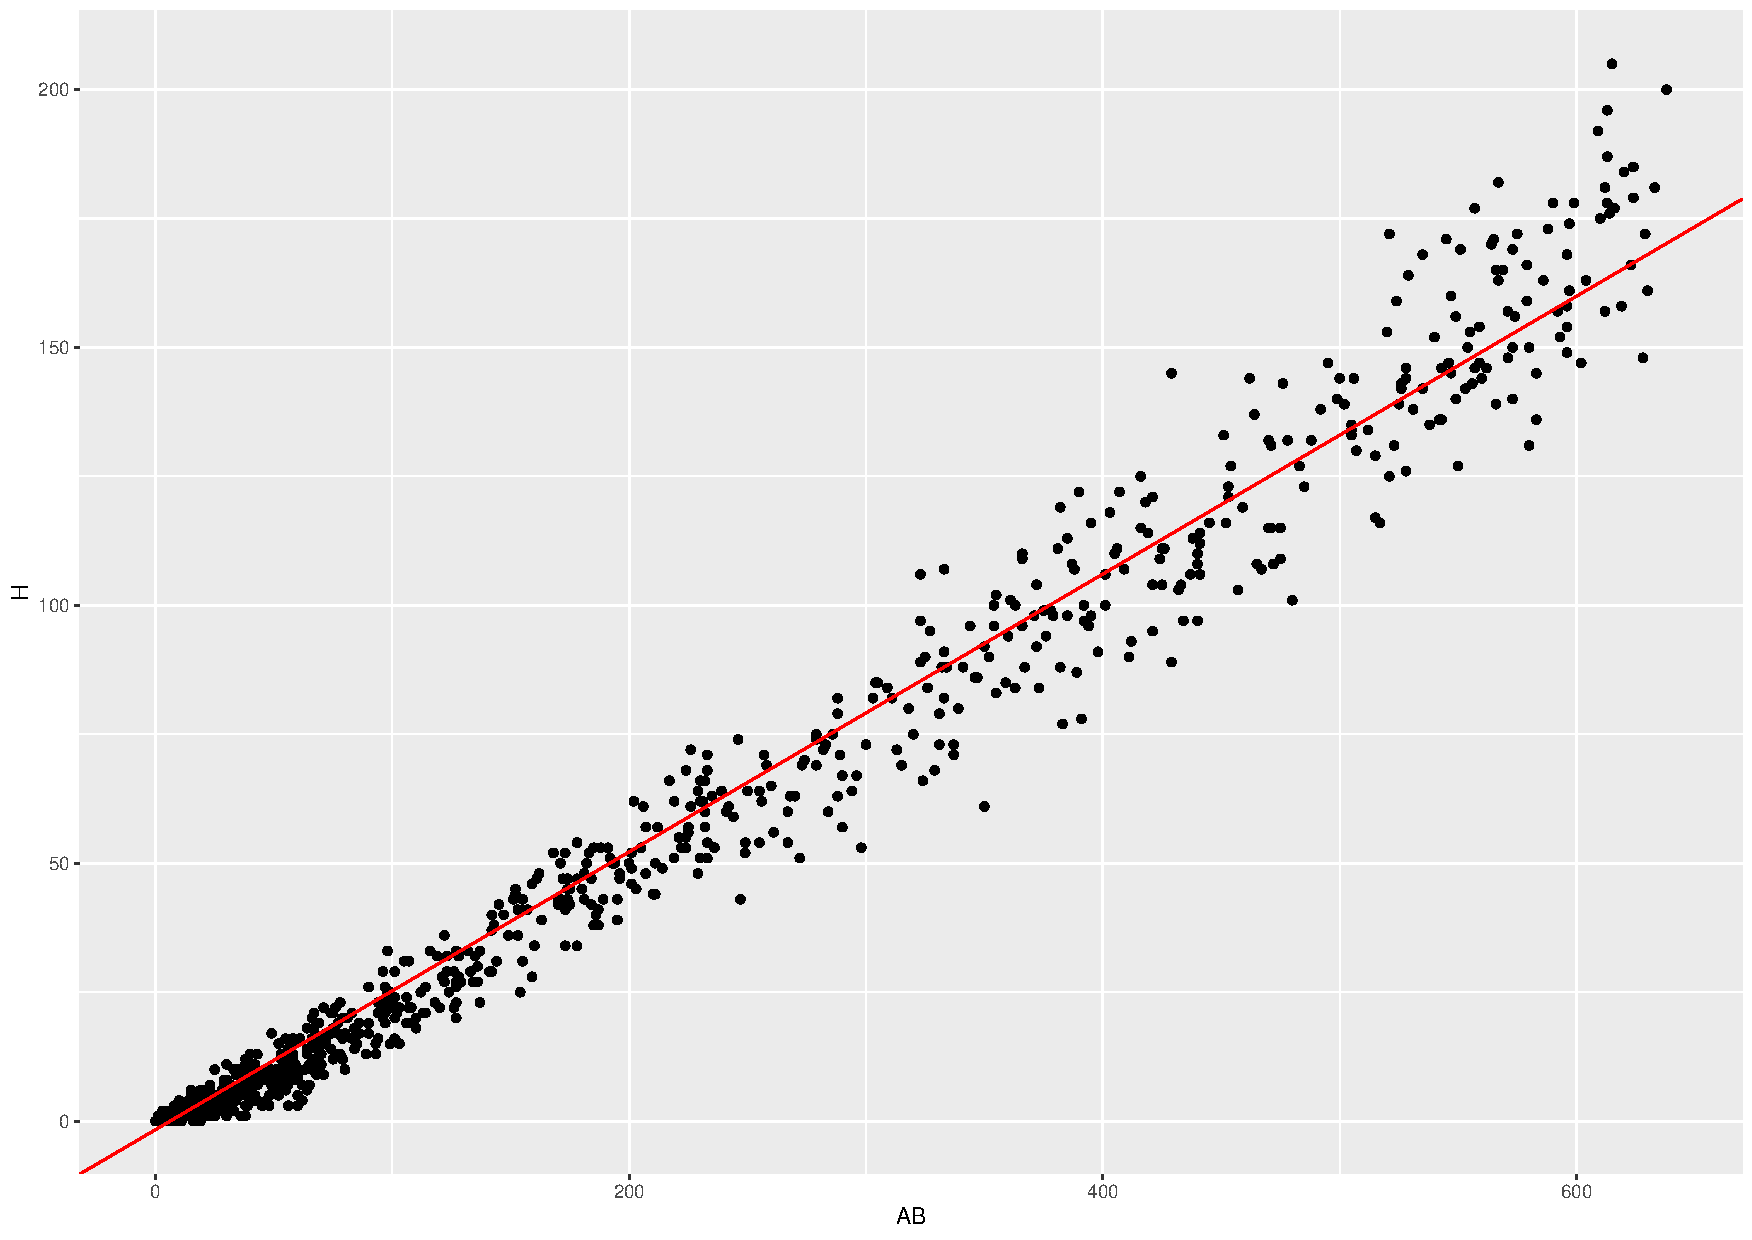
\includegraphics[width=10cm]{photographs/linreggg.pdf}
    \label{1}
\end{figure}
\bigskip
The plot we have produced (Plot 1) is displayed below with the regression line in red.
Clearly, we see that the more times a batter comes up to bat, the more likely it is for him to get a hit.

\subsubsection{Multi-variable Model}
Similar to above, we are able to construct a multi-variable model easily. What we need to do is to add more variables to the lm() function. We get the following syntax:

\begin{lstlisting}[basicstyle=\scriptsize]
lm.fit=lm(Hits~PlateApp + x2 + x3, data=Batting)
\end{lstlisting}




\section{Classification}
Classification is another popular method in predictive modelling. Unlike regression methods above, classification is more suited when you want to group data together to make predictions which are quantitative i.e. whether a patient has contracted a disease or not.

\subsection{Logistic Regression}
While the name suggests that this is a regression model, Logistic Regression (LR) is actually a classification model because its aim is using a regression model to predict an outcome between 0 and 1 and then categorize results based on the outcome. This outcome, in fact, is a probability model of the relationship between variables. 

\subsubsection{Mathematics of Logistic Regression}
In this case we can no longer use the formula above to predict the relationship because we would end up with negative probability which is not possible.
We aim to model the relationship as a probability where $p(X)$ = $P(Y = c|X = x)$ with $X$ the input variable and $Y$ the response variable with a target response $c$. \cite{CMULR}
Therefore we have to introduce a new formula called the \textbf{logistic function}:

\[p(X) = P(Y = 1|X = x) = \frac{\exp(\beta_0 + \beta_1X)}{1 + \exp(\beta_0 + \beta_1X)}\]\\
This formula is actually the Sigmoid function, $F(X) = \frac{\exp(x)}{1 + \exp(x)}$, where we have that $x = \beta_0 + \beta_1X$.

\begin{figure}[ht]
\centering
\begin{subfigure}{.5\textwidth}
  \centering
  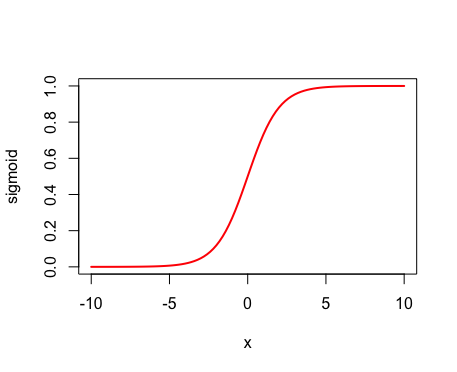
\includegraphics[width=7cm]{photographs/sigmoid.png}
  \caption{Sigmoid Function}
  \label{fig:sub1}
\end{subfigure}%
\begin{subfigure}{.5\textwidth}
  \centering
  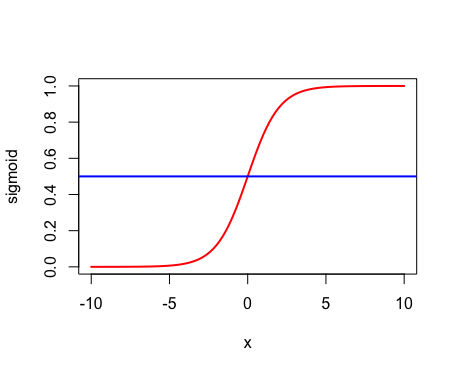
\includegraphics[width=7cm]{photographs/sigmoidline.png}
  \caption{Blue line to show classification boundary}
  \label{fig:sub2}
\end{subfigure}
\caption{How the Sigmoid function is used for logistic regression}
\label{fig:2}
\end{figure}
From this, we can rearrange this into an odds ratio between 0 and $\infty$, then take the logarithm to get the following:

\begin{equation}
\begin{split}
    \frac{p(X)}{1 - p(X)} &= \exp(\beta_0 + \beta_1X) \\
   \log\left(\frac{p(X)}{1 - p(X)}\right) &= \beta_0 + \beta_1X   
\end{split}
\end{equation}\\
Which turns out to be the equation of the \underline{linear regression model}! \cite[Section 4.4]{ESL}

\subsubsection{Multiple Logistic Regression}
Similar to the linear regression above, for multi-variable logistic regression, we extend it so that we have $x=\beta_0 + \sum_{i=1}^{n} X_i\beta_i$. We are able to use the same sigmoid function as in the 1-variable case because we have only changed the input $x$ by adding more variables.\\
Therefore we will have the following relation:
\[\log\left(\frac{p(X)}{1 - p(X)}\right) = \hat{\beta_0} + \sum_{i=1}^{n} X_i\hat{\beta_i}\]


\subsubsection{Calculating \textbf{$\beta_i$}}
To calculate $\beta_i$, we estimate $\hat{\beta_i}$ as we do in linear regression. However, instead of using non-linear least squares, we will use \textit{maximum likelihood} instead because Logistic Regressions involves predicting probabilities instead of just classes.\\
\bigskip
We will now follow on with calculations similar to \cite{CMULR}.\\
Say $c = 1$, [\textbf{Note:} Although this also works for $c > 1$ it is much messier so we stick with the simple case], then we establish the probabilities that:

\[ y_i = \left\{ \begin{array}{rcl}
        1 & \mbox{probability} & p \\
        0 & \mbox{probability} & 1-p
        \end{array}\right.
\]
The Likelihood is then:
\begin{equation}
    L(\beta_0, \beta) = \prod_{i=1}^{n} p(x_i)^{y_i} (1 - p(x_i))^{1 - y_i}
\end{equation}
And therefore the log-likelihood is:
\begin{equation}
    \begin{split}
        \ell(\beta_0, \beta) &= \sum_{i=1}^{n} y_i \log p(x_i) + (1 - y_i) \log (1 - p(x_i))\\
        &= \sum_{i=1}^{n} \log(1 - p(x_i)) + \sum_{i=1}^{n} y_i \log\left(\frac{p(x_i}{1 - p(x_i)}\right)\\
        &= \sum_{i=1}^{n} \left(-\log1 + e^{\beta_0 + \beta x_i}\right) + \sum_{i=1}^{n} y_i (\beta_0 + \beta x_i)
    \end{split}
\end{equation}
Which we differentiate to maximize:
\begin{equation}
    \diffp{\ell(\beta)}{\beta} = \sum_{i=1}^{n} x_i (y_i - p(x_i;\beta)) = 0
\end{equation}
To solve (3.8), we use Newton-Raphson methods evaluated at the previous $\beta$ to obtain a new $\beta$ until optimal.

\[
\beta^{new} = \beta^{old} - \left(\frac{\partial \ell(\beta)}{\partial \beta \partial \beta^\mathsf{T}}\right)^{-1} - \diffp{\ell(\beta)}{\beta}
\]

\subsubsection{Example}
We will look at the Teams data and try to create a logistic regression model based on the likelihood of the New York Yankees Team (NYA/NYY) winning the league. The variables we will be looking at are wins (W), runs scored (R), runs conceeded (ER) and hits (H). We will run all 4 factors at the same time and see how each affects the likelihood of winning the league.
\begin{lstlisting}[basicstyle=\scriptsize]
> library(Lahman)
> library("dplyr")
> library("ggplot2")
> teamseason <- Lahman::Teams

> nyaplayoff <- filter(teamseason, teamseason$teamID =="NYA")
> nyyplayoff <- nyaplayoff[c("W", "R", "ER", "H", "LgWin")]
> head(nyyplayoff)

   W   R  ER    H LgWin
1 72 579 411 1136     N
2 92 598 394 1354     N
3 71 586 440 1228     N
4 90 640 419 1354     N
5 70 605 449 1258     N
6 51 460 479 1190     N
\end{lstlisting}
Here we notice that the \underline{"LgWin"} column does not have numeric values which is needed. So we have to change this variable. In fact, due to a player strike in 1994, we also have a year where there was no winner and $\mathbf{<NA>}$ is also a factor which we need to remove. In fact we also see that the format of that column is not compatible with the function we will use and and has to be converted to an integer value.

\begin{lstlisting}[basicstyle=\scriptsize]
> nyyplayoff[nyyplayoff =="N"] = 0
> nyyplayoff[nyyplayoff =="Y"] = 1
> nyyplayoff %>% filter(!is.na(LgWin))
> head(nyyplayoff)
   W   R  ER    H LgWin
1 72 579 411 1136     0
2 92 598 394 1354     0
3 71 586 440 1228     0
4 90 640 419 1354     0
5 70 605 449 1258     0
6 51 460 479 1190     0
\end{lstlisting}

\begin{lstlisting}[basicstyle=\scriptsize]
> str(nyyplayoff)
'data.frame':	117 obs. of  5 variables:
 $ W    : int  72 92 71 90 70 51 74 88 76 50 ...
 $ R    : int  579 598 586 640 605 460 589 626 684 630 ...
 $ ER   : int  411 394 440 419 449 479 397 406 535 613 ...
 $ H    : int  1136 1354 1228 1354 1258 1190 1234 1254 1374 1320 ...
 $ LgWin: chr  "0" "0" "0" "0" ...
 
> nyyplayoff$LgWin <- as.integer(nyyplayoff$LgWin)
> str(nyyplayoff)
'data.frame':	117 obs. of  5 variables:
 $ W    : int  72 92 71 90 70 51 74 88 76 50 ...
 $ R    : int  579 598 586 640 605 460 589 626 684 630 ...
 $ ER   : int  411 394 440 419 449 479 397 406 535 613 ...
 $ H    : int  1136 1354 1228 1354 1258 1190 1234 1254 1374 1320 ...
 $ LgWin: int  0 0 0 0 0 0 0 0 0 0 ...
\end{lstlisting}
Now that all the values are integer values, we are able to run the logistic model on it and get the following results.

\begin{lstlisting}[basicstyle=\scriptsize]
> logreg <- glm(LgWin ~ ., data = nyyplayoff, family = "binomial")
> summary(logreg)

Call:
glm(formula = LgWin ~ ., family = "binomial", data = nyyplayoff)

Deviance Residuals: 
    Min       1Q   Median       3Q      Max  
-2.0175  -0.6131  -0.2235   0.7152   3.2710  

Coefficients:
              Estimate Std. Error z value Pr(>|z|)    
(Intercept) -14.625802   5.387761  -2.715 0.006635 ** 
W             0.170730   0.050386   3.388 0.000703 ***
R             0.002845   0.004948   0.575 0.565331    
ER           -0.011214   0.005052  -2.220 0.026442 *  
H             0.001609   0.004633   0.347 0.728346    
---
Signif. codes:  0 *** 0.001 ** 0.01 * 0.05 . 0.1  1

(Dispersion parameter for binomial family taken to be 1)

    Null deviance: 149.451  on 115  degrees of freedom
Residual deviance:  93.849  on 111  degrees of freedom
  (1 observation deleted due to missingness)
AIC: 103.85

Number of Fisher Scoring iterations: 6

\end{lstlisting}
We then are able to use this model to predict how another team, say the Boston Red Sox, would have done in a hypothetical season based on the parameters we have put into the model. We first prepare and extract the data exactly the same to that of the New York Yankees previously. Then add the following lines below.

\begin{lstlisting}[basicstyle=\scriptsize]
> lrprobs <- predict(logreg, newdata = teamplayoff[1:4], type = "response")
> lrpred <- ifelse(lrprobs > 0.5, "Win", "Lose")
\end{lstlisting}
Finally we can observe the predictions in both matrix form and graph form:

\begin{lstlisting}
> table(lrpred, teamplayoff$LgWin)
      
lrpred   0   1
  Lose 101   6
  Win    3   8
\end{lstlisting}

\begin{figure}[ht]
    \centering
    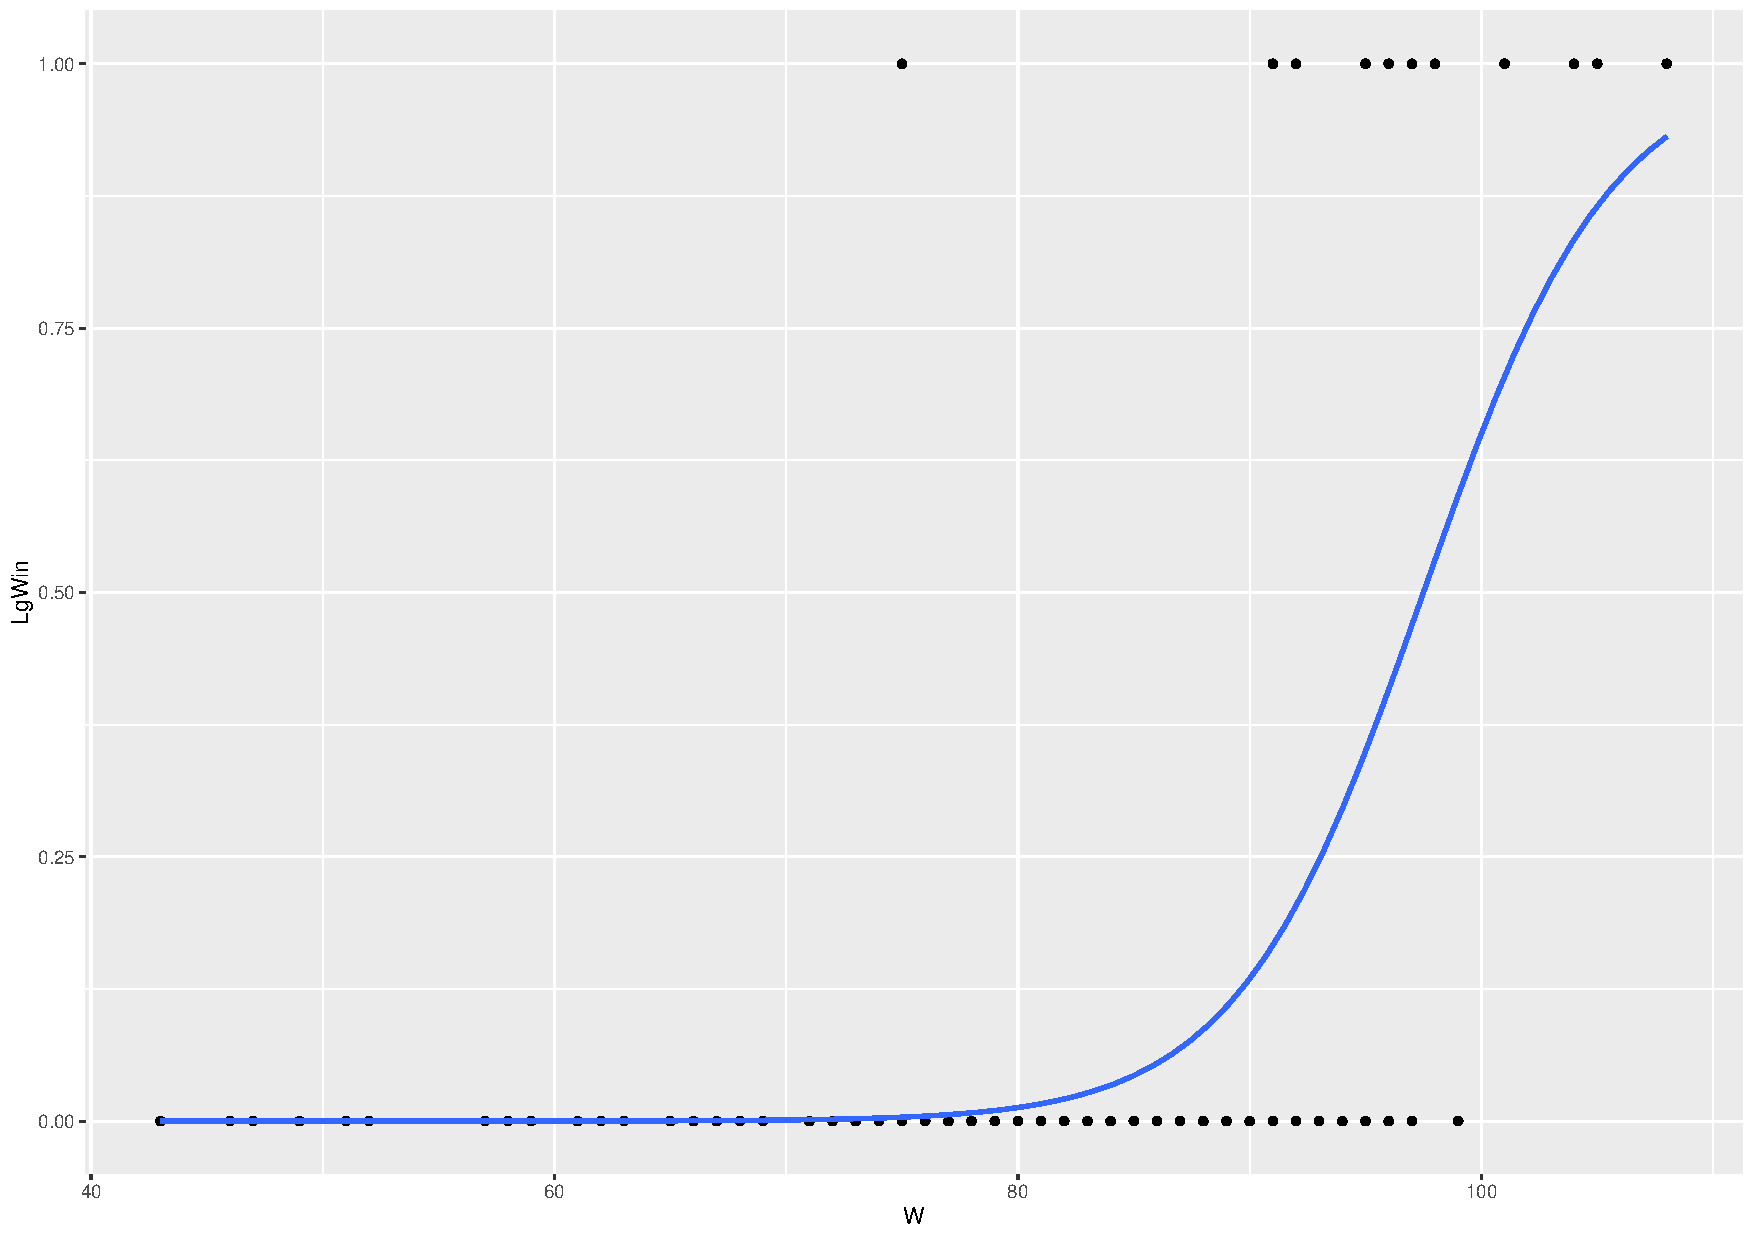
\includegraphics[width = 10cm]{photographs/logregpred.pdf}
    \caption{Predictions for the Boston Red Sox winning the League}
    \label{fig:log1}
\end{figure}




\chapter{Tree Models}
Having seen the basic statistical models, we can now look into building on from these simpler models. Ensemble learning looks at compiling multiple simple models to create a more robust model while reducing the likelihood of over-fitting the model. We first look at \textbf{Additive Modelling} which involved adding models onto models.

\subsubsection{Decision Trees}
The first method we look at is \textbf{Decision Trees} \cite{BreimanDT}. They work with both regression and classification models seen previously.
The idea of decision trees is to split up the data into segments (this is called \textit{segmenting}) and then keep breaking them down until we get suitable groups. This can then be summarized up into a tree which can be displayed to see the paths taken.
Decision trees are one of the most popular forms of supervised learning which is why it is the often the main base learner for ensemble methods which we will look at later.

\section{Basics on Decision Trees}
There are multiple methods used in Classification and Regression Trees. The most commonly used are: CART, C4.5, and ID3, among others. \\
A general idea is to think of a continuous variable $Y$ and some inputs $X_i ,  i = 0,...,n$. Lets say for simplicity, we have for two variables $X_1, X_2$ (thus creating a 2-D plane), we are able to create two separate regions from a partition, which we then model $Y$ on. This partition is on either $X_1$ or $X_2$. \\
Then, we are able to repeat the process for either one or both regions and model $Y$ on the new partitions and continue to do so until we get to a stopping point.

We can also represent this as a tree model with the branches descending from the top. This is often how we present decision trees as they are very easy to interpret even without much knowledge of statistics.



The first question we ask is \underline{how do we know where to split each branch the tree?}
\bigskip

In fact, we find there are \textbf{two} major metrics that are used in deciding where to split each branch.

\begin{enumerate}
    \item \textbf{\textit{Gini Impurity}}: Used by the CART method, 
    
    \item \textbf{\textit{Information Gain}}: Used in methods such as C4.5, ID3
\end{enumerate}

\subsection{Calculating metrics}
We find that both are based on the idea of Entropy, which itself is part of \textbf{Information Theory}, defined by Claude E. Shannon in 1948 in his landmark paper "A Mathematical Theory of Communication". \footnote{http://cm.bell-labs.com/cm/ms/what/shannonday/shannon1948.pdf} \cite{Shannon}.

\begin{definition}[Entropy]\cite{Shannon}
The Entropy of a random variable is defined as the information uncertainty in the variable's possible outcomes.
\end{definition}
In fact, Shannon had formulated this into a theorem for entropy which we will now state:
\begin{theorem}[Entropy] [Based on source \cite[Section 6, p. 10]{Shannon}]\\
For a measure $H(p_1,\dots,p_n)$ where $p_1 + \dots + p_n = 1$ with the following conditions:
\begin{enumerate}
    \item $H$ is continuous in $p_i$
    
    \item If all $p_i$'s are equal, then $H$ is monotonic
    
    \item If a choice is broken down into two successive choices, then $H$ becomes the sum of each individual values.\\
    \textbf{For Example}: $H(\frac{1}{2}, \frac{2}{5}, \frac{1}{10}) = H(\frac{1}{2}, \frac{1}{2}) + \frac{1}{2}H(\frac{4}{5}, \frac{1}{5})$
\end{enumerate}
If the above is satisfied, we can define entropy as:
\begin{equation}
    H(T) = I_E (p_1, \dots , p_n) = -\sum_{i=1}^{n} p_i \log_b p_i
\end{equation}
\end{theorem}
In this case we have to derive two forms of entropy:

\begin{enumerate}
    \item Entropy of one attribute (Parent Entropy):
    \begin{equation}
        H(T) = -\sum_{i=1}^{n} p_i \log_2 p_i
    \end{equation}
    This is the full data
    
    \item Entropy of two attributes (Child Entropy):
    \begin{equation}
       H(T \mid a) = -\sum_{i=1}^{n} P(i \mid a) \log_2 P(i \mid a) 
    \end{equation}
    This is the filtered data and the sum of each Child Entropy is equal to the Parent Entropy
\end{enumerate}
We then use the two entropy's to calculate information gain.

\begin{definition}[Information Gain]
Information Gain can be defined as the following:
\begin{equation}
    IG(T,a) = E(T) - E(T \mid a)
\end{equation}
\end{definition}
Information Gain is used to decide on which feature to split on. We want it so that each split provides the most "information" and is therefore the value with this highest $IG(T,a)$. If $IG(T,a) = 0$, then we have found a leaf node and stop, else repeat the process until we arrive at a leaf node.\\
This is used in ID3 and C4.5. We will come back to this later when we progress onto more additive models

\medskip
Due to the nature for calculating information gain, if you were only doing a basic decision tree, we would use a much simpler algorithm called CART.\\
CART uses a method called \textbf{Gini Impurity} which measures how often we would incorrectly sort a random element from the set. 

\begin{definition}[Gini Impurity]\footnote{https://en.wikipedia.org/wiki/Decision\_tree\_learning}
Based off Tsallis Entropy, the Gini Impurity can be defined as the following:
\begin{equation}
    I_G (p) = I_G (p_1, \dots, p_n) = 1 - \sum_{i=1}^{n} p_i^2
\end{equation}
\end{definition} \cite[Metrics]{TreeWiki}

\subsection{Algorithm for Decision Trees}



\section{Regression Trees}
There are two major algorithms which are used for CART:

\begin{itemize}
    \item tree \cite{tree} - The basic decision tree algorithm in R
    \item rpart \cite{rpart} - The Open Source CART algorithm developed to replace tree
\end{itemize}

\subsection{Salaries Example}
Baseball has some of the higest salaries in all of sports and we are able to use Regression Trees to figure out how much a player should earn based on similar attributes.
\begin{figure}
    \centering
    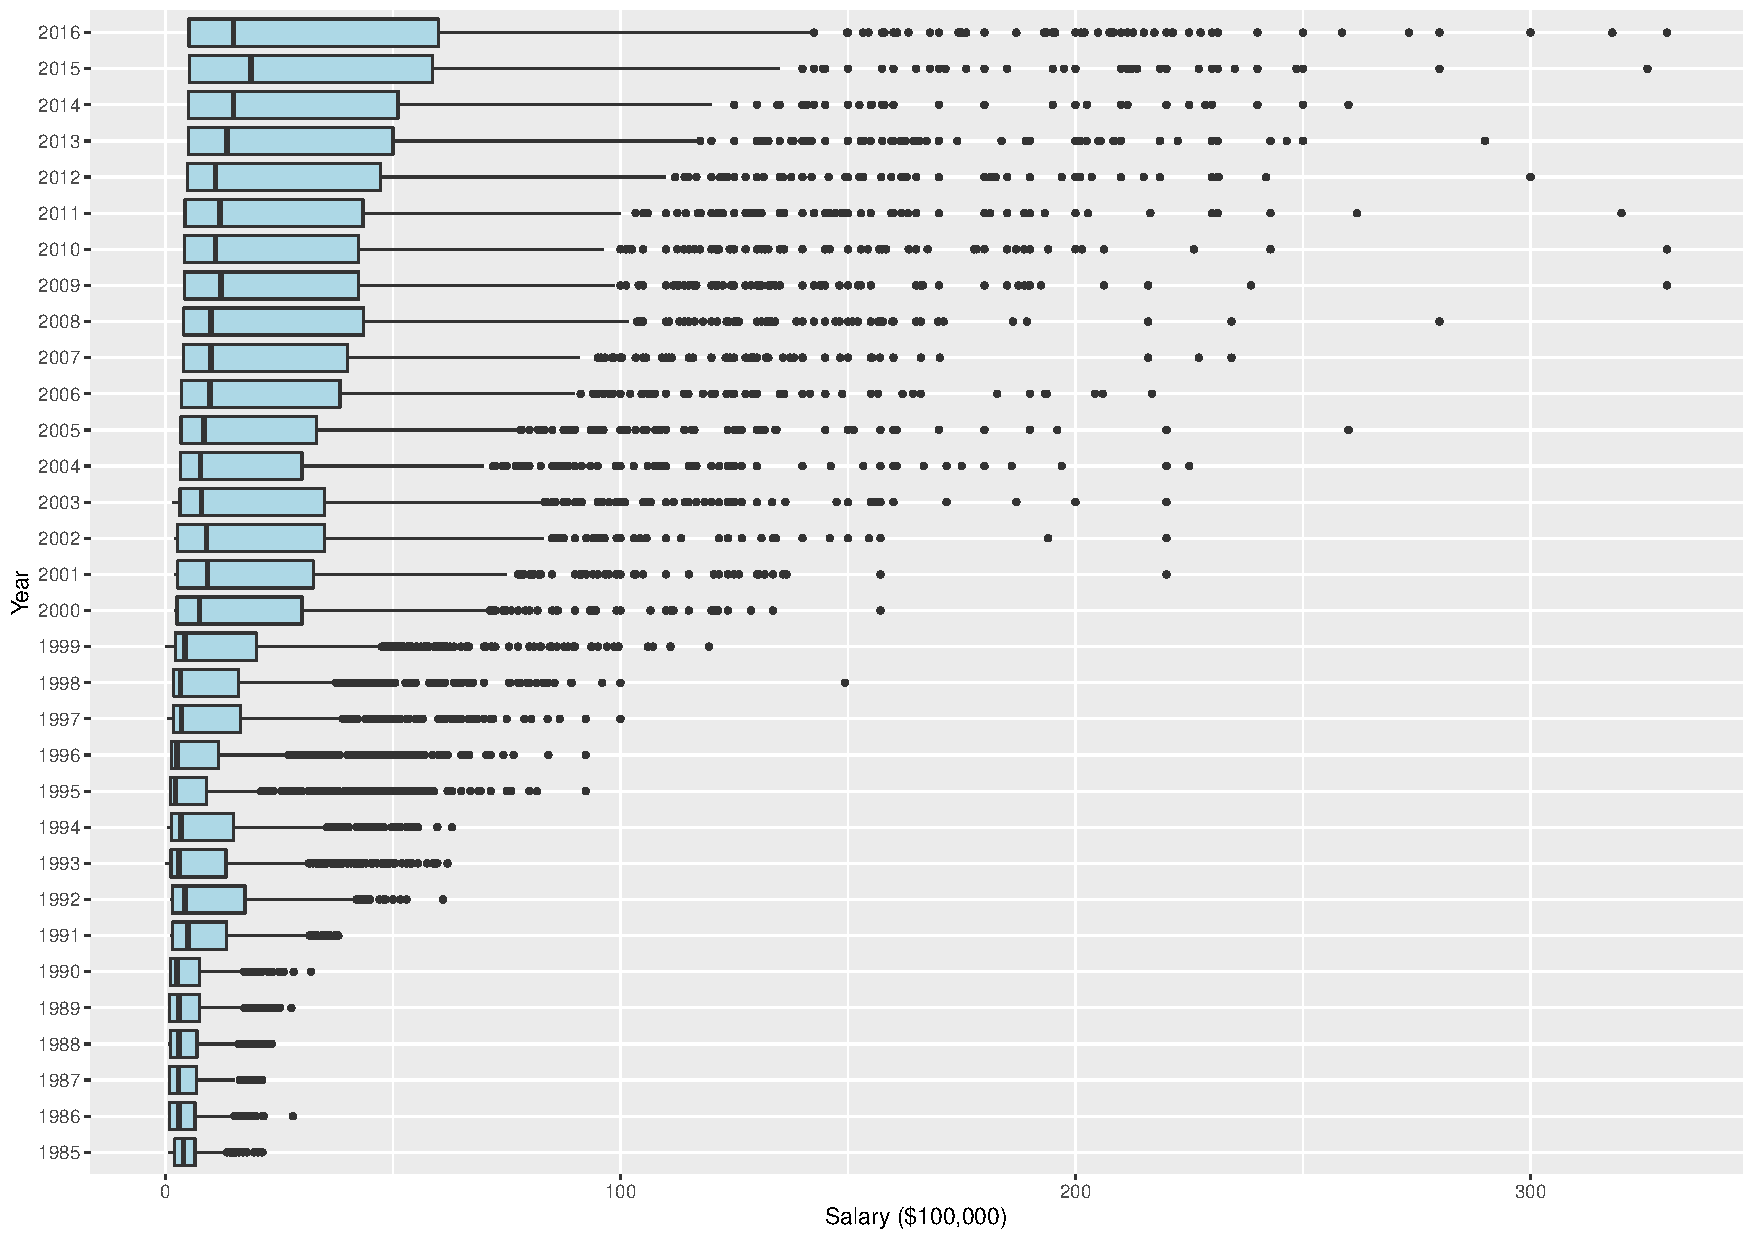
\includegraphics[width = 12cm]{photographs/Salaries.pdf}
    \caption{Baseball Salary Spread over the years}
    \label{fig:salaries}
\end{figure}\\
We will be observing players from the year 2005 onwards in this analysis to reduce the likelihood of overfitting the model because salaries earlier than 2000 tend to be much lower as a consequence of the changing value of money over time.\\
\medskip
We firstly have to merge two data tables (Batting and Salaries) to obtain all the data needed to do this analysis. From there, we can proceed as normal with the following lines of code along with the usual Lahman, ggplot2 and dplyr libraries:

\begin{lstlisting}[basicstyle=\scriptsize]
> library(rpart) #Cart method
> library(rpart.plot)

> ggplot(Salaries, aes(x = factor(yearID), y = salary/1e5)) +
+   geom_boxplot(fill = "lightblue", outlier.size = 1) +
+   labs(x = "Year", y = "Salary ($100,000)") +
+   coord_flip()
> batting <- Batting %>%
+   filter(yearID >= 1985) %>%
+   left_join(select(Salaries, playerID, yearID, teamID, salary), 
+             by=c("playerID", "yearID", "teamID"))
> str(batting)

> batting <- batting %>%
+   filter(yearID >= 2005)

> batting %>%
+   filter(! is.na(salary))

> salreg <- rpart(formula = salary ~ yearID + G + AB + R + 
+   H + X2B + HR + RBI + SB + BB + SO + GIDP, data = batting, 
+   method = "anova", control = list(minsplit = 10, maxdepth = 10, xval = 10))
\end{lstlisting}

A basic raw decision tree can be obtained from here. However, to produce better plots, the function rpart.plot which is a part of rpart \cite{rpart} can be used to obtain Figure 4.2:

\begin{lstlisting}[basicstyle=\scriptsize]
> salreg
n=9633 (11795 observations deleted due to missingness)

node), split, n, deviance, yval
      * denotes terminal node

 1) root 9633 2.113174e+17 3487293  
   2) RBI< 61.5 8314 1.423508e+17 2973140  
     4) AB< 1.5 2628 1.884897e+16 2065544 *
     5) AB>=1.5 5686 1.203366e+17 3392620  
      10) G>=35.5 3417 5.295648e+16 2859599  
        20) RBI< 28.5 1736 1.485619e+16 1941948 *
        21) RBI>=28.5 1681 3.512875e+16 3807275 *
      11) G< 35.5 2269 6.494729e+16 4195322 *
   3) RBI>=61.5 1319 5.291526e+16 6728133 *
   
> rpart.plot(salreg)
\end{lstlisting}

\begin{figure}
\centering
\begin{subfigure}{.5\textwidth}
    \centering
    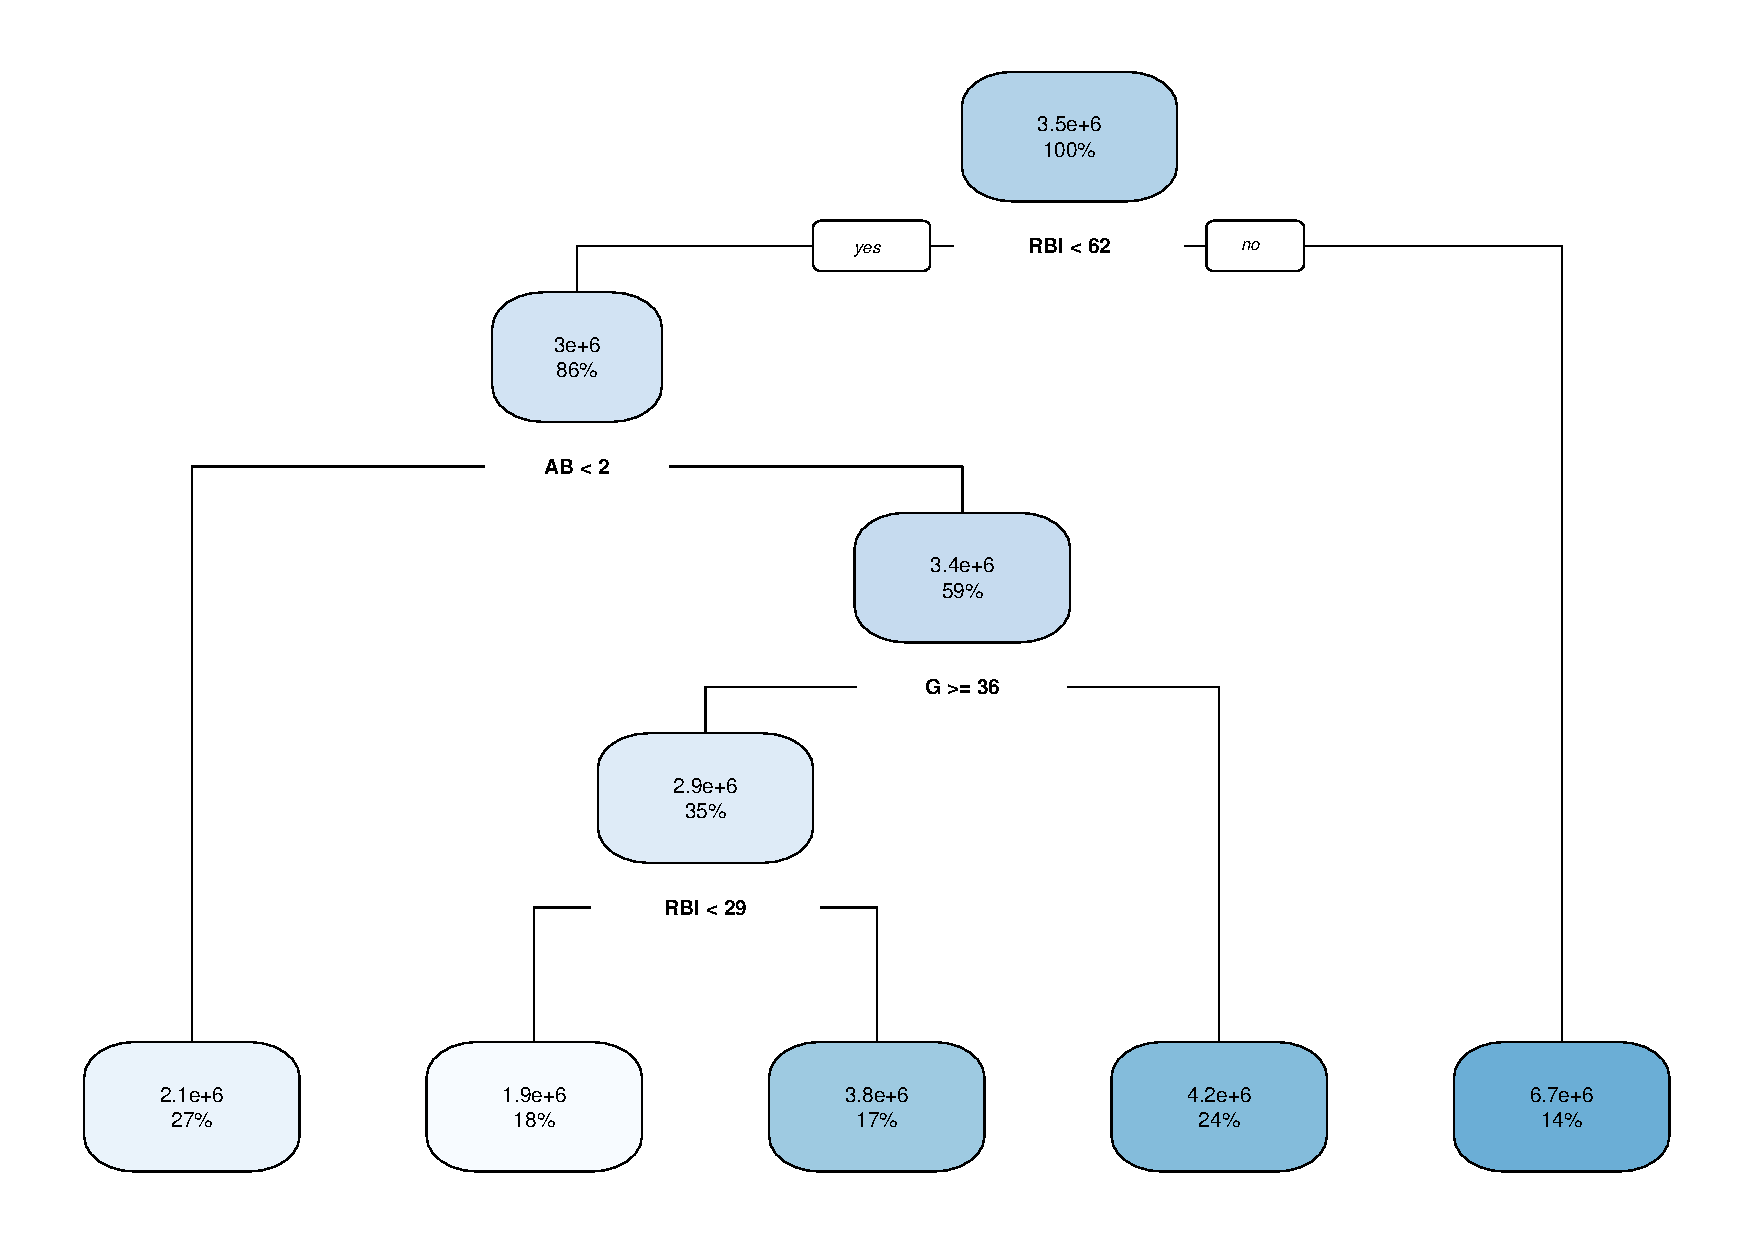
\includegraphics[width = 7cm]{photographs/regtree2005.pdf}
    \caption{Regression Tree from rpart.plot}
    \label{fig:regplot}
\end{subfigure}%
\begin{subfigure}{.5\textwidth}
    \centering
    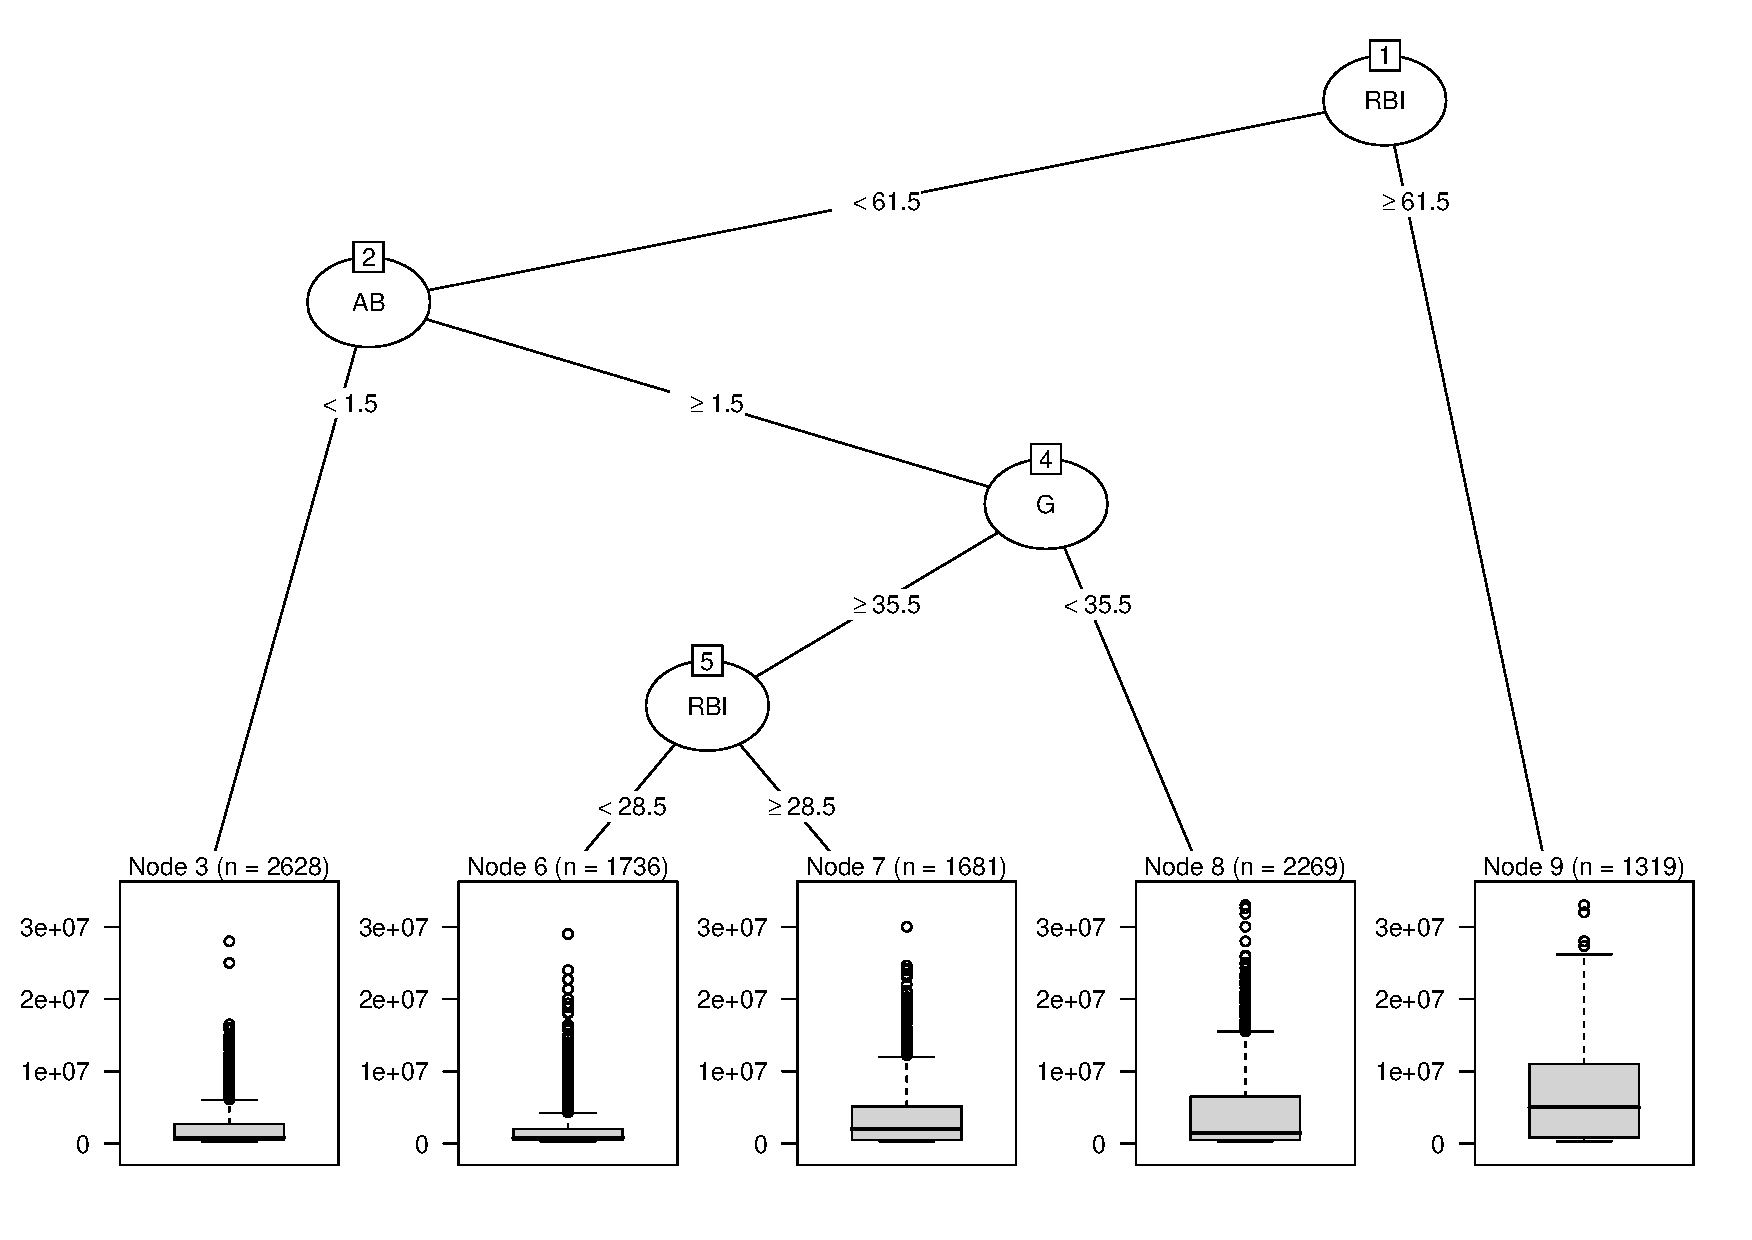
\includegraphics[width = 7cm]{photographs/regparty.pdf}
    \caption{Using Rparty to show information on each group}
    \label{fig:regparty}
\end{subfigure}
\caption{Regression Tree Plots for Salaries 2005-2015}
\label{fig:regtree}
\end{figure}

\begin{figure}
\centering
\begin{subfigure}{.5\textwidth}
    \centering
    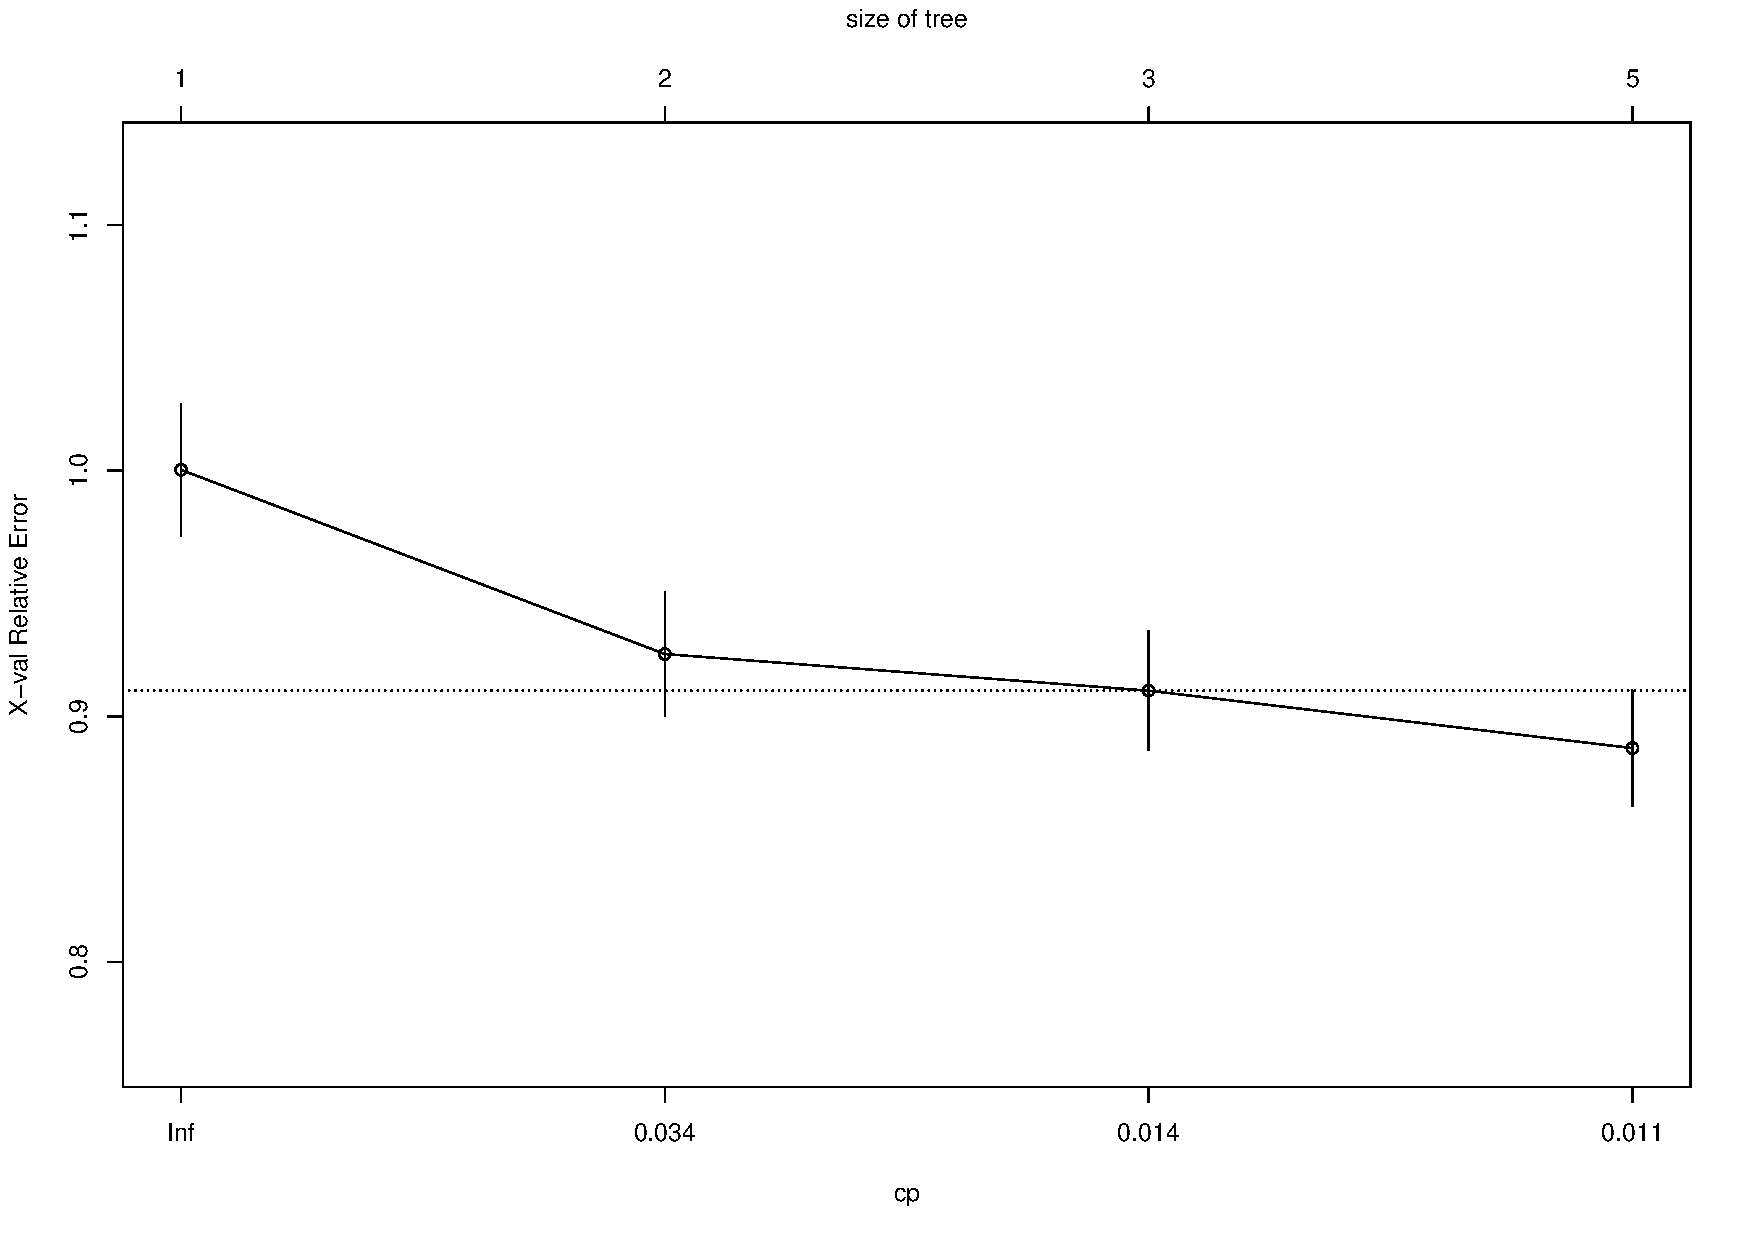
\includegraphics[width = 7cm]{photographs/regerror.pdf}
    \caption{Error of Regression Tree by Size}
    \label{fig:regerror}
\end{subfigure}%
\begin{subfigure}{.5\textwidth}
    \centering
    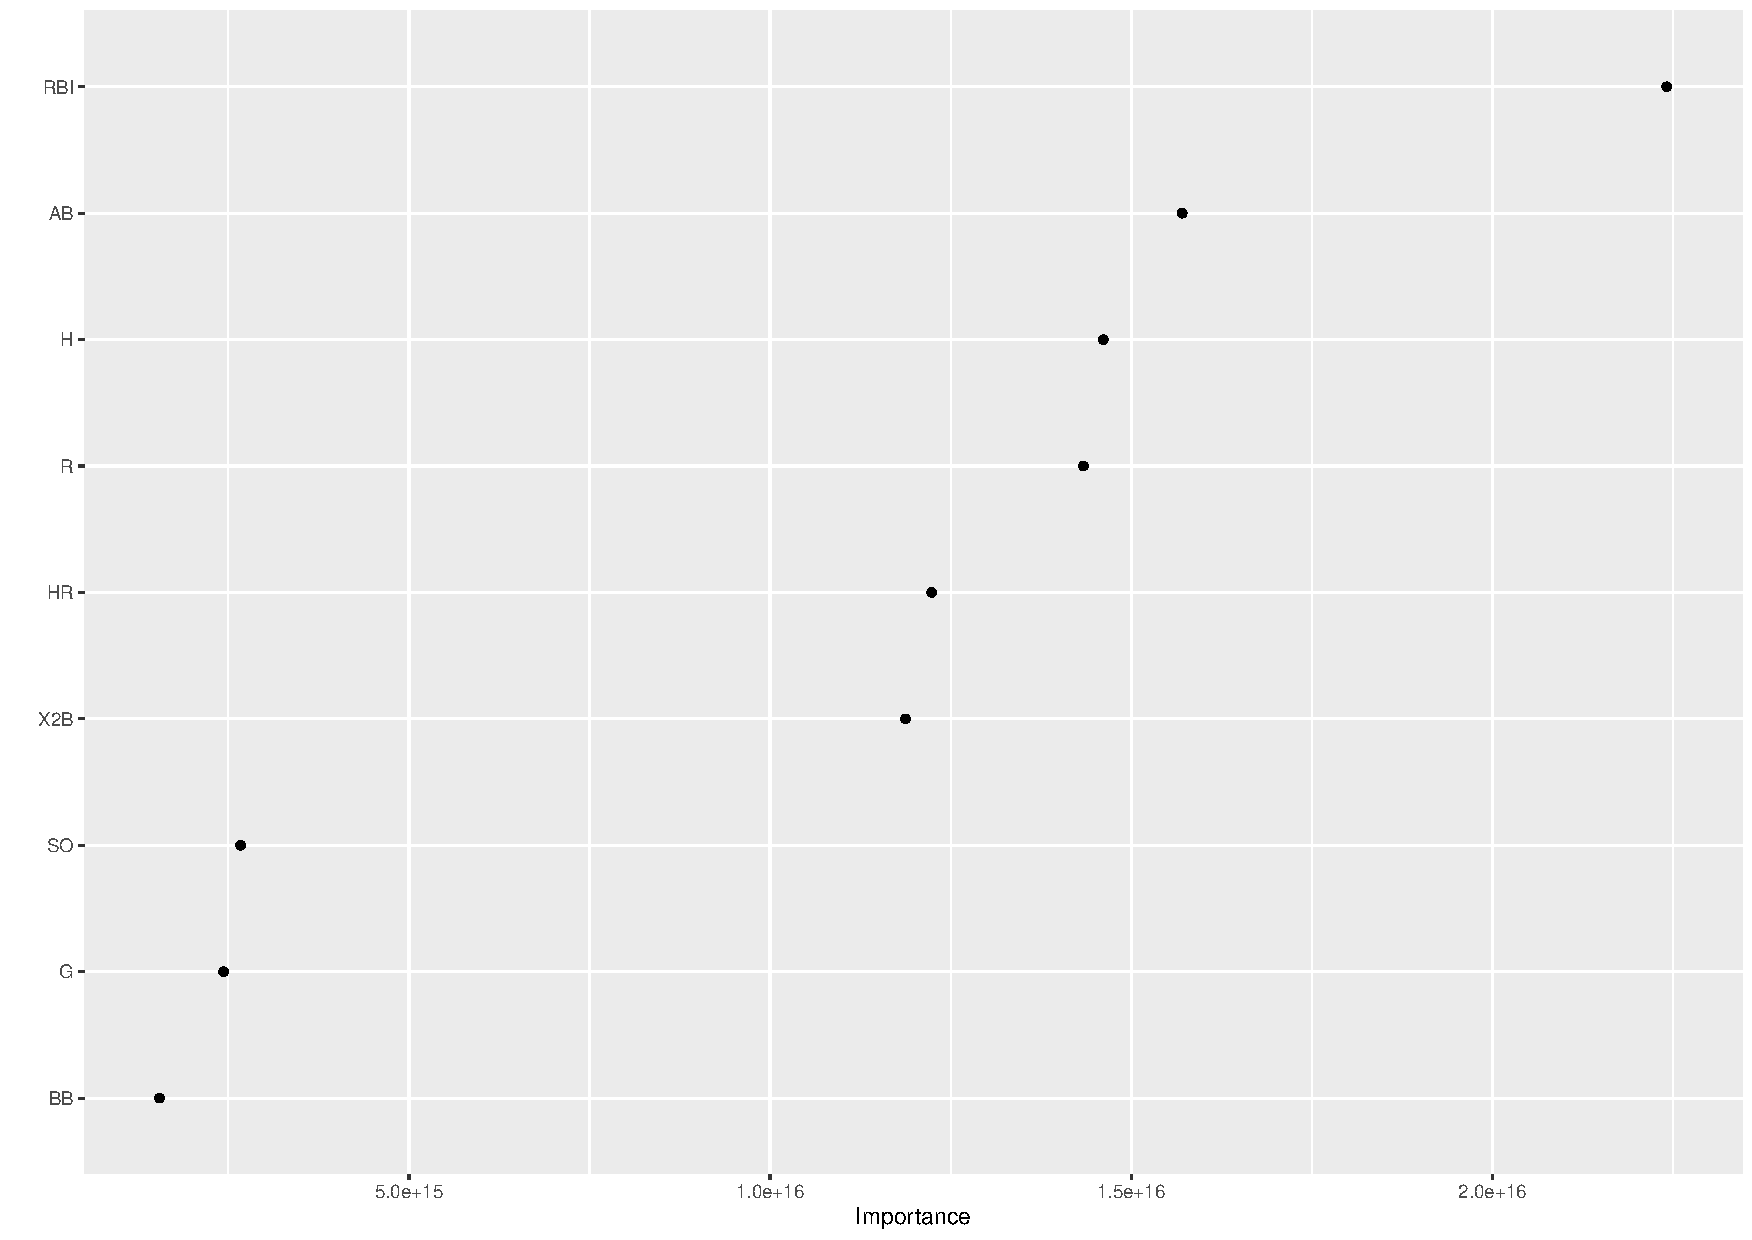
\includegraphics[width = 7cm]{photographs/regimportance.pdf}
    \caption{Feature Importance}
    \label{fig:regimp}
\end{subfigure}
\caption{Extra information on how the algorithm calculated where to split}
\label{fig:regsidedata}
\end{figure}

To see how the algorithm works, here is part of the summary for the tree model we have made above.

\begin{lstlisting}[basicstyle=\scriptsize]
> summary(salreg)
Call:
rpart(formula = salary ~ yearID + G + AB + R + H + X2B + HR + 
    RBI + SB + BB + SO + GIDP, data = batting, method = "anova", 
    control = list(minsplit = 10, maxdepth = 10, xval = 10))
  n=9633 (11795 observations deleted due to missingness)

          CP nsplit rel error    xerror       xstd
1 0.07595846      0 1.0000000 1.0002293 0.02687708
2 0.01497883      1 0.9240415 0.9249818 0.02495898
3 0.01278725      2 0.9090627 0.9100690 0.02421890
4 0.01000000      4 0.8834882 0.8869111 0.02344675

Variable importance
RBI  AB   H   R  HR X2B  SO   G  BB 
 23  16  15  15  13  12   3   2   2 

Node number 1: 9633 observations,    complexity param=0.07595846
  mean=3487293, MSE=2.193683e+13 
  left son=2 (8314 obs) right son=3 (1319 obs)
  Primary splits:
      RBI < 61.5   to the left,  improve=0.07595846, (0 missing)
      BB  < 42.5   to the left,  improve=0.07244418, (0 missing)
      HR  < 10.5   to the left,  improve=0.06611753, (0 missing)
      R   < 55.5   to the left,  improve=0.06595827, (0 missing)
      H   < 98.5   to the left,  improve=0.06104507, (0 missing)
  Surrogate splits:
      HR  < 17.5   to the left,  agree=0.951, adj=0.641, (0 split)
      R   < 61.5   to the left,  agree=0.936, adj=0.534, (0 split)
      AB  < 478.5  to the left,  agree=0.935, adj=0.526, (0 split)
      H   < 126.5  to the left,  agree=0.934, adj=0.517, (0 split)
      X2B < 24.5   to the left,  agree=0.931, adj=0.498, (0 split)

\end{lstlisting}
We see here that the split RBI $<$ 61.5 provides the higest improvement for Gini Impurity and is thus the branch chosen to be split over all other splits.



\section{Classification Trees}
For a classification example, we will try to classify baseball players based on whether they would make the Baseball Hall of Fame or not.\\
For full disclosure I am not the first person to do this and in fact, this has been done on baseballwithr previously \cite{hofclass}. I thank the author of that article for providing the code which this Classification Tree is based off.


\begin{figure}[ht]
    \centering
    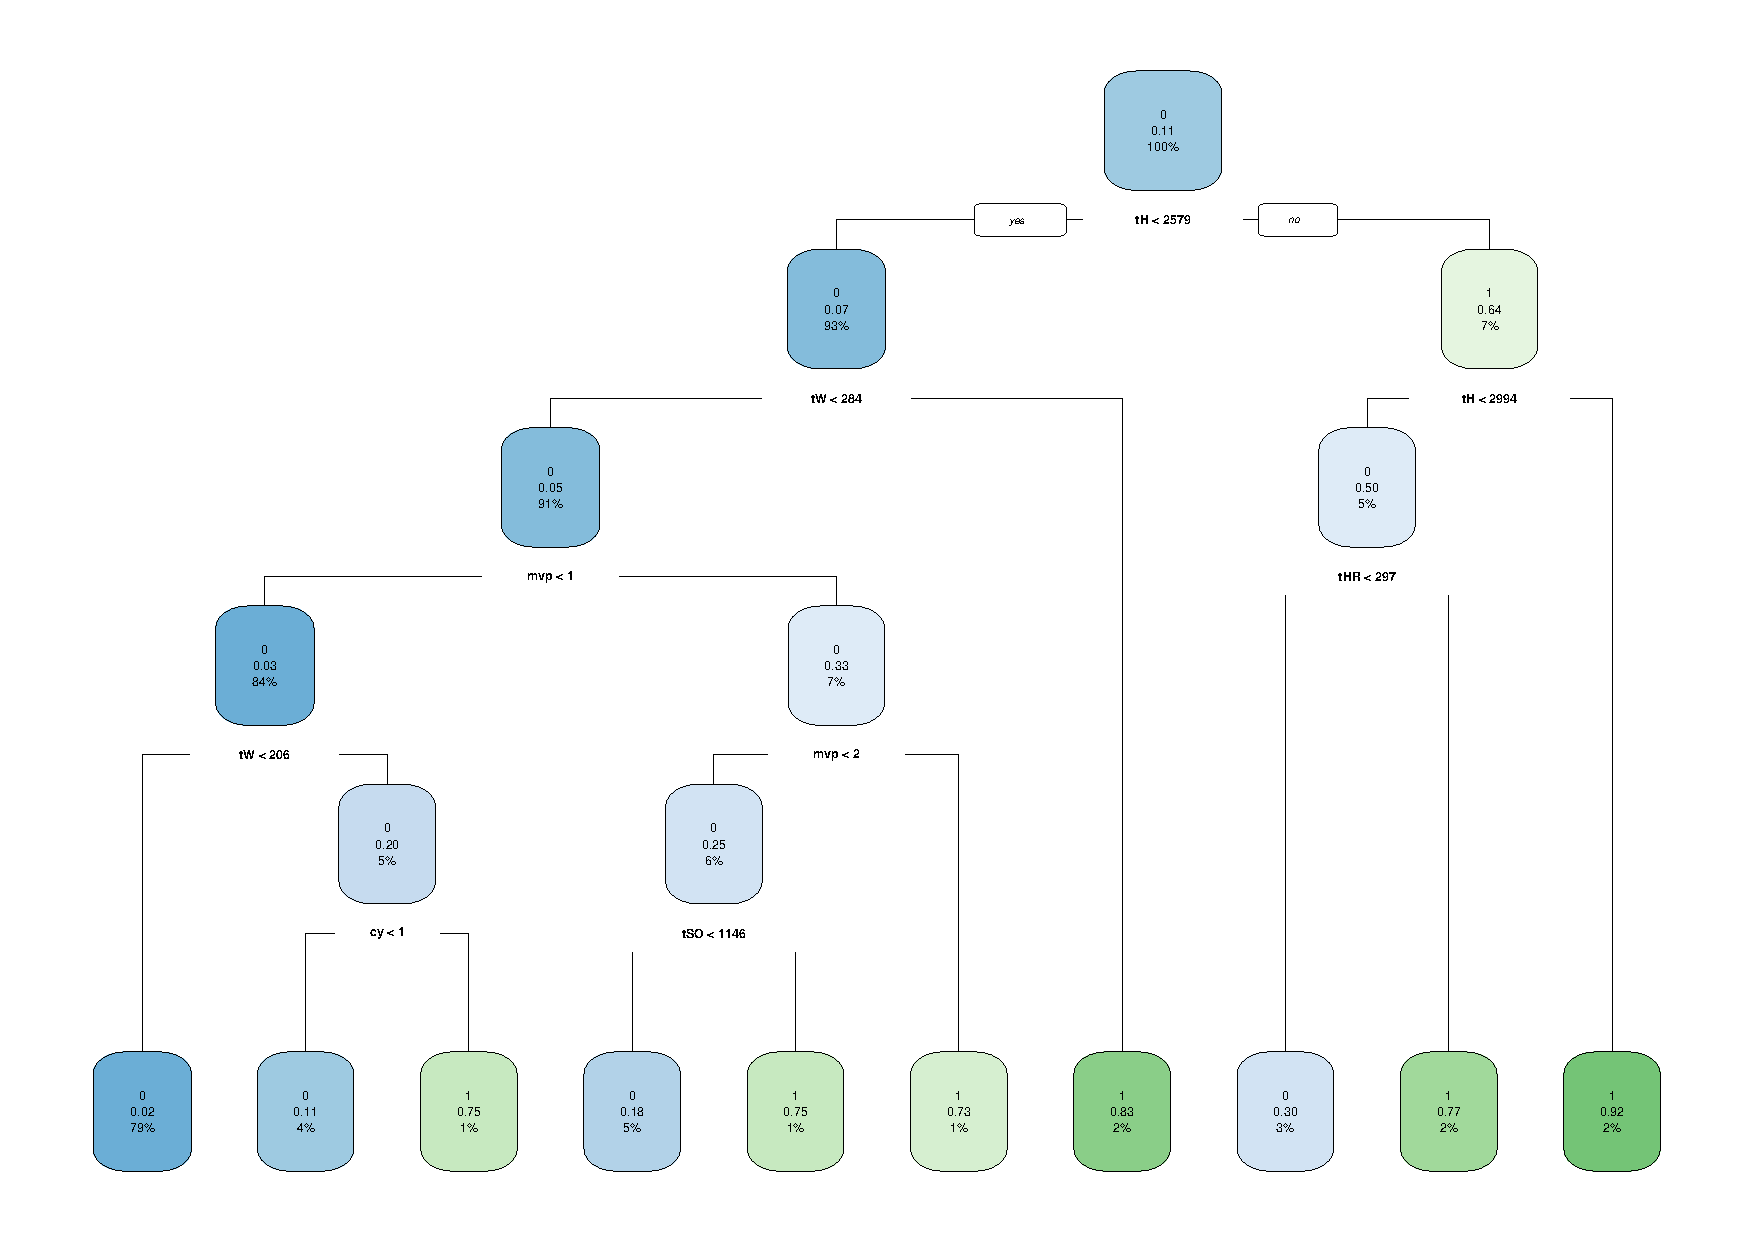
\includegraphics[width = 12cm]{photographs/hofclass.pdf}
    \caption{Classification Tree on whether a player made the Hall of Fame}
    \label{fig:hof}
\end{figure}

\chapter{Bagging and Random Forest}
Not content with the flaws of CART, Leo Breiman started working on methods to improve on and ended up with two methods which are closely linked and follow on from each other. While many others tried to improve metric selections, they tend to have their own flaws which make them less useful than CART. Breiman figured out that bootstrapping techniques \cite{bootstrap} were the most efficient method, in the 1990s in terms of computer power, while also providing an improvement over CART.
\bigskip\\
The first is \textbf{B}ootstrap \textbf{Agg}regat\textbf{ing} (Bagging) \cite{bagging} \footnote{As an aside, the editor of that paper was Ross Quinlan, the same person who invented ID3, C4.5} which uses bootstrapping techniques to generate many trees to aggregate. Here, all $n$ features are selected as possible splitting nodes for trees and we \textit{aggregate} all trees to build our model.
\medskip\\
The next stage improvement was \textbf{Random Forests} \cite{randomforest}.
Random Forest uses bootstrapping techniques to train multiple weak learners which create a much stronger model when combined together.
Indeed Random Forests only differ from Bagging in the selection of features as Random Forests only select a subset of features and "vote" on the best features when aggregating the final model.
\bigskip\\
These technique are called \textbf{Ensemble Learning} and will come up again since they are the most common methods to improving accuracy on decision trees.
Note that while these methods do allow us to reduce the chance of overfitting the data compared to regular Decision Tree methods, they do not eliminate them and it is still possible for overfitting to occur although the prevalence of multiple bootstrapping samples averaging each other out does reduce the chance of overfitting occuring.

\section{Bagging}
Bootstrap Aggregating (Bagging) involves using multiple learning samples from the $\{x_{i}, y_{i}\}_{i=1}^{n}$ dataset, we collectively denoted these as $\mathcal{L}$. 
We denote each bootstrap sample as $\mathcal{L}_k$ where $k \in [1, \dots, B]$.\\
The aim here is to get an aggregated predictor, made up of individual predictors $\varphi_k$ which is better than the individual predictor, which we will denote the final predictor as $\varphi$. 
This is achieved by taking the average of the bootstrap samples:

\[ \varphi = av_{k = 1,\dots,B} (\varphi_k) \]

In theory, this bagged estimator is:
\begin{equation}
    \varphi = \frac{1}{B} \sum_{k=1}^{B} \varphi_k
\end{equation}
Thus we can define Bagging as follows:
\begin{definition}[Bagging]
    A tree-based method comprised of $B$ \textit{randomly} bootstrapped, independent and identically distributed, samples where the final predictor is formed by aggregating all $B$ samples 
\end{definition}
Each bootstrap is drawn at random and with replacement and thus it is possible for repeated trees to occur. 
Thus stronger decision points would tend to outweigh weaker trees as they pull the average towards these decisions.
\medskip\\
We will now follow on from Leo Breiman's paper \cite{bagging} for the procedure needed.

\subsection{Classification}
For each individual tree, we use the same method to construct them as we had previously.
The following procedure is followed for all runs:
\begin{algorithm}
\begin{enumerate}
    \item A seed is set to allow for replication
    
    \item The full dataset is split \textit{randomly} into a learning set $\mathcal{L}$ and a testing set $\mathcal{T}$
    
    \item A Classification Tree is constructed from the full $\mathcal{L}$ and the test set $\mathcal{T}$ is run to test the misclassification rate
    
    \item 50 bootstrap sample from $\mathcal{L}$ are drawn randomly, and each make a $\phi$ classifier to form $\phi_1, \dots, \phi_{50}$
    
    \item All 50 $\phi$ classifiers are compared with each other and the most common classifier is selected, else, the class with the lowest error relative to the full Classification Tree is selected and this becomes $\varphi_k$
    
    \item Repeat steps 4-5 $k$ times and average the $\varphi_k$ values to obtain $\varphi$
\end{enumerate}
\caption{Classification Bagging}
\end{algorithm}



\subsection{Regression}
Similarly, we use an almost identical meta-algorithm to classification but with some minor differences.
The following procedure is followed for all runs:
\begin{algorithm}
\begin{enumerate}
    \item A seed is set to allow for replication
    
    \item The full dataset is split \textit{randomly} into a learning set $\mathcal{L}$ and a testing set $\mathcal{T}$
    
    \item A Regression Tree is constructed from the full $\mathcal{L}$ and the test set $\mathcal{T}$ is run to test the misclassification rate
    
    \item 50 bootstrap sample from $\mathcal{L}$ are drawn randomly, and each make a $\phi$ regression to form $\phi_1, \dots, \phi_{50}$
    
    \item Here, the predictor is $\hat{y}_k = av\phi_k$ is used instead of $\varphi$ where we have the squared error $av(y_n - \hat{y}_n)^2$
    
    \item Repeat steps 4-5 $k$ times and average the $\hat{y}_k$ values to obtain $\varphi$
\end{enumerate}
\caption{Regression Bagging}
\end{algorithm}


\subsection{Implementations of Bagging}
There are two ways one could implement bagging. The first is using the \texttt{bagging} function from the \texttt{ipred} library \cite{ipred}. 
This is a version which relies on \texttt{rpart} from earlier and does not require much data prep. 
\bigskip\\
An alternative version is using \texttt{randomForest} \cite{Rforest} and setting \texttt{mtry = m} where \texttt{m} is the number of variables we have in the data we want to perform bagging on.
\bigskip\\
These two versions do not prove to differ by much and are essentially identical in the grand scheme of things, as they usually differ from different samples being bootstrapped.
However you may prefer to use \texttt{randomForest} if you were to be also performing a Random Forest at the same time. 


\section{Random Forests}
Random Forests are a natural development from Bagging as they use very similar techniques for growing ensembles. 
In his paper \cite{randomforest}, which will be replicated here, he noted that while both Bagging and Random Forests are similar, Bagging is akin to "\dots darts thrown at random boxes \dots", Random Forests are much more civilized in nature as they are formed by voting "\dots for the most popular class."\\
In fact the trees we grow are actually formed and trained using bagging methods we have described earlier.


\subsection{Convergence of Random Forests}
We firstly show that Random Forests converge.
We begin by using Breiman's definition of what a Random Forest is \cite{randomforest}:
\begin{definition}[Random Forests]
    A tree-based method formed from $k$, $k \in \mathbb{N}$, independent and identically distributed ensemble of classifiers, $h_1, \dots , h_k$.\\
    Each tree casts one vote for the most popular class which is to be selected.
\end{definition}
We have that $h_{k_i}$ is the classifier we get from sample $k$ from the full dataset $\{x_i, y_i\}_{i=1}^{n}$. 
Here, as always, we use two different metrics for classification and regression:
\subsubsection{Classification}
We can define the margin function, which measures the average number of votes for the class $k_1$ over all other classes $k_i$, $i \neq 1$, with indicator $I$ as 
\begin{definition}[Margin of Random Forests]
   \[ mg(x, y) = av_k I (h_{k_1}) - \max_{k_i \neq k_1} av_k I (h_{k_i}) \] 
\end{definition}

We aim to maximise the margin as this shows that the ensembles are more likely to agree with what is a strong split compared to weaker splits.

\subsubsection{Regression}
Here, unlike previously, we used the mean-squared error instead of the residual sum-squared:
\begin{definition}[Mean-Squared Generalization Error]
    Given the vector $y_{k_i}$ made up of the true values from the selected $x_{k_i}$ variables, the mean-squared generalization error is
    \[ E(y_{k_i} - h_{k_i})^2 \]
\end{definition}

\subsection{Random Forest Algorithm}
Using the above metrics, we can now give the meta-algorithm for the Random Forest Algorithm. Note that it is in fact very similar to the algorithm for Bagging as we are using Bootstrapping to select individual ensemble trees which we are aiming to use in our final model.
\subsubsection{Algorithm}
\begin{algorithm}
\SetAlgoLined
\begin{enumerate}
    \item A seed is set to allow for replication
    
    \item Draw $B$ bootstrapped samples from the learning set $\mathcal{L}$
        
    \item Grow a random forest as follows:
    \begin{enumerate}
        \item Select $m$ variables randomly from the sample $\mathcal{L}_b$ where $b \in [1, \dots, B]$
        
        \item Form a regular decision tree using only the selected features and the relevant metric described above
        
        \item Output the classifiers $\phi_1, \dots, \phi_B$
    \end{enumerate}
    
    \item Make a prediction as follows
    \begin{description}
        \item[Regression] $ \frac{1}{B} \sum_{b=1}^{B} \phi_b $
        
        \item[Classification] $majority \{\phi_b\}_{b=1}^{B}$
    \end{description}
\end{enumerate}
\caption{Random Forest Algorithm}
\end{algorithm}
Here, we note the following when choosing the preferred optimal value of $m$ (For which \texttt{randomForest} does this automatically if undefined by the user):
\begin{itemize}
    \item \textbf{Classification} - $m = \left \lfloor{\sqrt{p}} \right \rfloor$ with minimum node size one
    
    \item \textbf{Regression} - $m = \left \lfloor{\frac{p}{3}} \right \rfloor$ with minimum node size five
\end{itemize}

\subsubsection{Out of Bag Samples}
The \textbf{Out of Bag Samples} (OOB) is used to check how good how well a model is fitted. 
A feature of selecting only a certain sample for bootstrapping is that we can use the samples not selected for a certain bootstrap to be a testing variable. 
Thus if variable $\{x_i, y_i\} \notin \mathcal{L}$ we can construct a predictor for this variable from the trees in which this variable is not a training data in.
\bigskip\\
We are able to use this value to tell us right away if a model is good as a good model would have a low OOB value. 
This is helpful as \texttt{R} calculates the OOB value for us automatically and if a bad model were to be found to have been fitted, we can discover this early on before proceeding onwards towards predicting values.

\subsection{Example}


\chapter{Boosting}
Boosting is a more modern method of ensemble learning and is based on the philosophy of additive learning - forming a complex model by adding lots of simple learners\footnote{https://towardsdatascience.com/demystifying-maths-of-gradient-boosting-bd5715e82b7c}.\\
\bigskip
The first modern meta-algorithm used for boosting was called \textbf{Adaptive Boosting} (commonly called AdaBoost) [Freund and Schapire], however, recently the newer meta-algorithm of \textbf{Gradient Boosting} [Friedman, 1999] has become the more preferred method mainly in part due to the \textbf{XGBoost} library which works for many languages including Python, R, Julia, Java, and C++. Another modern library is LightGBM by Microsoft [Ke, 2016] which is based on decision tree algorithms.

\chapter{Boosting}
\textbf{Boosting} is the next progression onwards from Random Forests.
There are many implementations of Boosting Algorithms presently available including AdaBoost, Gradient Boosting, xgBoost, LightGBM etc.
We will focus on the two most famous implementations, AdaBoost \cite{adaboost}, and Gradient Boosting \cite{gbm} along with a modern extension of this, xgBoost \cite{xgboost}.
While Boosting is similar to Random Forests, there are some subtle differences which make them much more accurate and optimal in terms of making predictions.

\subsubsection{Difference Between Boosting and Bagging/RF}
While the previously seen methods of Bagging and Random Forests work on Bootstrapping samples and running many trees at the same time before aggregating/voting for results, Boosting involves using many "weak learners" which learn from incorrect predictions. 
Here, incorrect learners are sampled more often and given more weight when learning to improve on these mistakes and try to minimize the errors that these weak learners produce.
The final model is formed from combining all the weak learners into a much stronger single model.


\section{AdaBoost}
The first modern boosting model is the \textbf{Adaptive Boosting} (AdaBoost) model. Freund and Schapire had both independently developed basic boosting algorithms , but they were not optimal and thus they combined to work on AdaBoost which resolved most of the issues that had occured in previous attempts \cite{adaboost}.
\medskip\\
The idea \cite{adasummary} is to have $t = [1,\dots,T]$ \textit{weak learners} - which consist of small one-step decision trees referred to as stumps - and maintain weight over each training variable $x_i$ in the training set.
The weight for training variable $i$ on weak learner round $t$ is denoted $w_t (i)$, and is initially set the same for all models before being updated after each round $t$. The weight is adjusted so that the variables which have been {\color{red} \underline{incorrectly classified}} are given more weight for the $t+1$ round. We will first formulate this as a classification problem before extending it for regression.

\subsection{Adjusting for Incorrect Classification}

\subsubsection{Error of Weak Hypothesis}
The job of the weak learner is to find a weak hypothesis $h_t : X \rightarrow \{-1,+1\}$ for $x_i \in X$ suitable for $w_t$ \cite{adasummary}. How good the hypothesis is can be tested by its error $\varepsilon_t$.
\begin{equation}
   \varepsilon_t = \sum_{h_t (x_i) \neq y_i} w_t (i) 
\end{equation}
In computations there exists a function called \textbf{WeakLearn} which achieves this by using \textit{decision stumps}.

%%Hedge
\subsubsection{Hedge/Weighted Majority Algorithm}
The \textbf{Hedge}, also known as the \textbf{Weighted Majority} \cite{wma} is an algorithm used to update the weighting of variables to decide which variable we should focus on when doing the next round $t + 1$. 
In our case, we use an adapted algorithm from Littlestone and Warmuth which Freund and Schapire called \textbf{Hedge($\beta$)} with the following distribution vector.
\begin{equation}
   \textbf{p}_t = \frac{\textbf{w}_t}{\sum_{i=1}^{n} w_t (i) } 
\end{equation}
Where $\textbf{w}^t$ is the vector of weights.
The following algorithm shows us how to update the Hedge($\beta$) after each turn:

\begin{algorithm}
\SetAlgoLined
\textbf{Parameters}:
\begin{description}
    \item $\beta \in [0,1]$
    \item Initial Weight Vector $\textbf{w}_1 \in [0,1]^n$ with $\sum_{i=1}^{n} w_1 (i) = 1$
    \item number of trials $T$
\end{description}
\For{$t = 1,\dots,T$}{
Choose Allocation \[ \frac{\textbf{w}_t}{\sum_{i=1}^{n} w_t (i)} \] \\
Incure Loss Vector $\ell^t \in [0,1]^n $ leading to loss $\textbf{p}^t \ell^t$ \\
Set New Weight to be 
\[ w_{t+1} (i) = w_t (i) \beta^{\ell_t (i)}
\] 
}
\caption{Hedge}
\end{algorithm}
\textbf{Note:} In fact, we can adapt this to the scenario where we have $\ell = \left|h_t(x_i) - y_i \right|$ and $\beta = \frac{\varepsilon}{1 - \varepsilon}$ and already achieve our AdaBoost with the following return:
\[
h_f (x) = 
\begin{cases}
1, & \text{if } \sum_{t=1}^T \left(\log \frac{1}{\beta^t} \right) h_t (x) \geq \frac{1}{2} \sum_{t=1}^T \left(\log \frac{1}{\beta^t} \right) \\
0, & \text{otherwise}
\end{cases}
\]
However, computationally, this is not preferred and a much more efficient algorithm is used when re-scaling the weightings.

\subsection{AdaBoost Algorithm for Classification}
\begin{algorithm}
\SetAlgoLined
\begin{enumerate}
    \item Set $\textbf{w}_1 = \frac{1}{n}$ $\forall$ $n$ training sets
    
    \item \For{$t = 1,\dots,T$}{
    Pick $h_t$ which minimizes $\varepsilon_t = \sum_{h_t (x_i) \neq y_i} w_t (i) $ \\
    Compute weight of chosen classifier 
    \[\alpha_t = \frac{1}{2} \log \frac{1 - \varepsilon_t}{\varepsilon_t} \] \\
    Update weights
    \[ w_{t+1} (i) = \frac{w_t (i) \exp{-\alpha y_i h_t (x_i)}}{Z_t} \]
    Where $Z_t$ is the normalization factor \\
    Break if $\varepsilon_t = 0$ or $\varepsilon_t \geq \frac{1}{2}$
    }
    
    \item Output final hypothesis
    \[ h_f (x) = \text{sign} \left(\sum_{t=1}^T \alpha_t h_t (x) \right) \]
\end{enumerate}
\caption{AdaBoost}
\end{algorithm}



\subsection{AdaBoost are Random Forests}
When comparing AdaBoost with Random Forests, one wonders whether the improvements between models are worth comparing. Indeed this was noted by Breiman in his Random Forests paper \cite{randomforest} suggests that these two methods are very similar. In fact Breiman made the following conjecture which we will call a theorem:
\begin{theorem}
AdaBoost is a Random Forest
\end{theorem}
The "proof" of this will be left to the reader to consult \cite{randomforest}

\section{Gradient Boosting}
Gradient Boosting was developed by Jerome Friedman \cite{gbm} and is similar to AdaBoost, but relies on the idea of \textbf{gradient descent} 
\subsection{Gradient Boosting Machines}


\section{Flowchart Showing Model Building}
\begin{tikzpicture}[->,>=stealth']
    % Start
    \node[state] (Data)
    {\begin{tabular}{l}
        \textbf{Data Set} 
    \end{tabular}}
    
    \node[state,
    node distance=6cm,     
    text width=3cm,        
    right of= Data,        
    yshift=+3cm] (Train)
    {\begin{tabular}{l}
        \textbf{Training Data}
    \end{tabular}
    }
    
    \node[state,
    node distance=6cm,     
    text width=3cm,        
    below of= Train,        
    yshift=-3cm] (Test)
    {\begin{tabular}{l}
        \textbf{Testing Data}
    \end{tabular}
    }
    
\end{tikzpicture}


\bibliographystyle{apalike}
\bibliography{reference}

\end{document}
